\section{Thiết kế}

\subsection{Hình ảnh thiết kế hình dáng 3D của sản phẩm}

Vỏ hộp sản phẩm được thiết kế trên phần mềm Autodesk Fusion 360 và chế tạo bằng công nghệ in 3D nhựa ABS. Kích thước tổng thể của vỏ hộp là $150 \times 100 \times 47\text{ mm}$, độ dày vách $2.5\text{ mm}$ và nắp $3.0\text{ mm}$. Cấu trúc gồm hai phần: Thân hộp (Bottom Case) và Nắp hộp (Top Cover), liên kết bằng khớp ngàm cài và 4 vít M3. Bên trong hộp có vách ngăn tách biệt khoang vi điều khiển ESP32 và khoang cảm biến nhiệt ẩm DHT22 có khe thông gió riêng, nhằm hạn chế nhiệt lượng tỏa ra từ vi điều khiển làm ảnh hưởng đến độ chính xác của cảm biến.

\begin{center}
\scriptsize
\renewcommand{\arraystretch}{0.92}
\begin{tabular}{|c|p{4.2cm}|p{5.5cm}|c|}
\hline
\textbf{STT} & \textbf{Vị trí bố trí trên vỏ hộp 3D} & \textbf{Chi tiết khoét lỗ / Gia công cơ khí} & \textbf{ID Chức năng} \\ \hline
1 & Màn hình LCD 1602 mặt trên & Khoét cửa sổ chữ nhật $71.0 \times 24.0\text{ mm}$ & \textbf{ID 5} \\ \hline
2 & Nút nhấn cơ học đổi trạng thái & Khoét lỗ tròn $\varnothing 7.0\text{ mm}$ cách mép phải $15\text{ mm}$ & \textbf{ID 6} \\ \hline
3 & Đèn LED đỏ báo tập trung & Khoét lỗ xuyên $\varnothing 5.2\text{ mm}$ viền vát $45^\circ$ & \textbf{ID 6} \\ \hline
4 & Vùng cảm ứng quẹt thẻ RFID & Khu vực $52 \times 34\text{ mm}$ dán sát mặt dưới nắp (đọc xuyên 3mm) & \textbf{ID 2} \\ \hline
5 & Đầu đón sáng quang trở LM393 & Khoét lỗ tròn $\varnothing 5.5\text{ mm}$ đón quang thông & \textbf{ID 4} \\ \hline
6 & Còi báo âm thanh Active Buzzer & Cụm 5 lỗ tròn thoát âm $\varnothing 1.5\text{ mm}$ & \textbf{ID 3} \\ \hline
7 & Khe cảm biến nhiệt ẩm DHT22 & 4 khe thông khí $12.0 \times 2.0\text{ mm}$ vách hông & \textbf{ID 1} \\ \hline
8 & Khoang vi điều khiển ESP32 & 4 trụ đỡ ốc vít M3 có ren đồng cấy nhiệt ở đáy & \textbf{ID 11, ID 12} \\ \hline
9 & Cổng cấp nguồn Micro USB & Khoét lỗ vát bo tròn $12.0 \times 7.0\text{ mm}$ ở vách sau & Cấp nguồn \\ \hline
\end{tabular}
\captionof{table}{Bảng ánh xạ vị trí lắp đặt linh kiện trên vỏ hộp 3D với ID chức năng}
\label{tab:map_3d_chuc_nang}
\end{center}

\begin{center}
\captionsetup{type=figure}
    \begin{subfigure}[b]{0.46\textwidth}
        \centering
        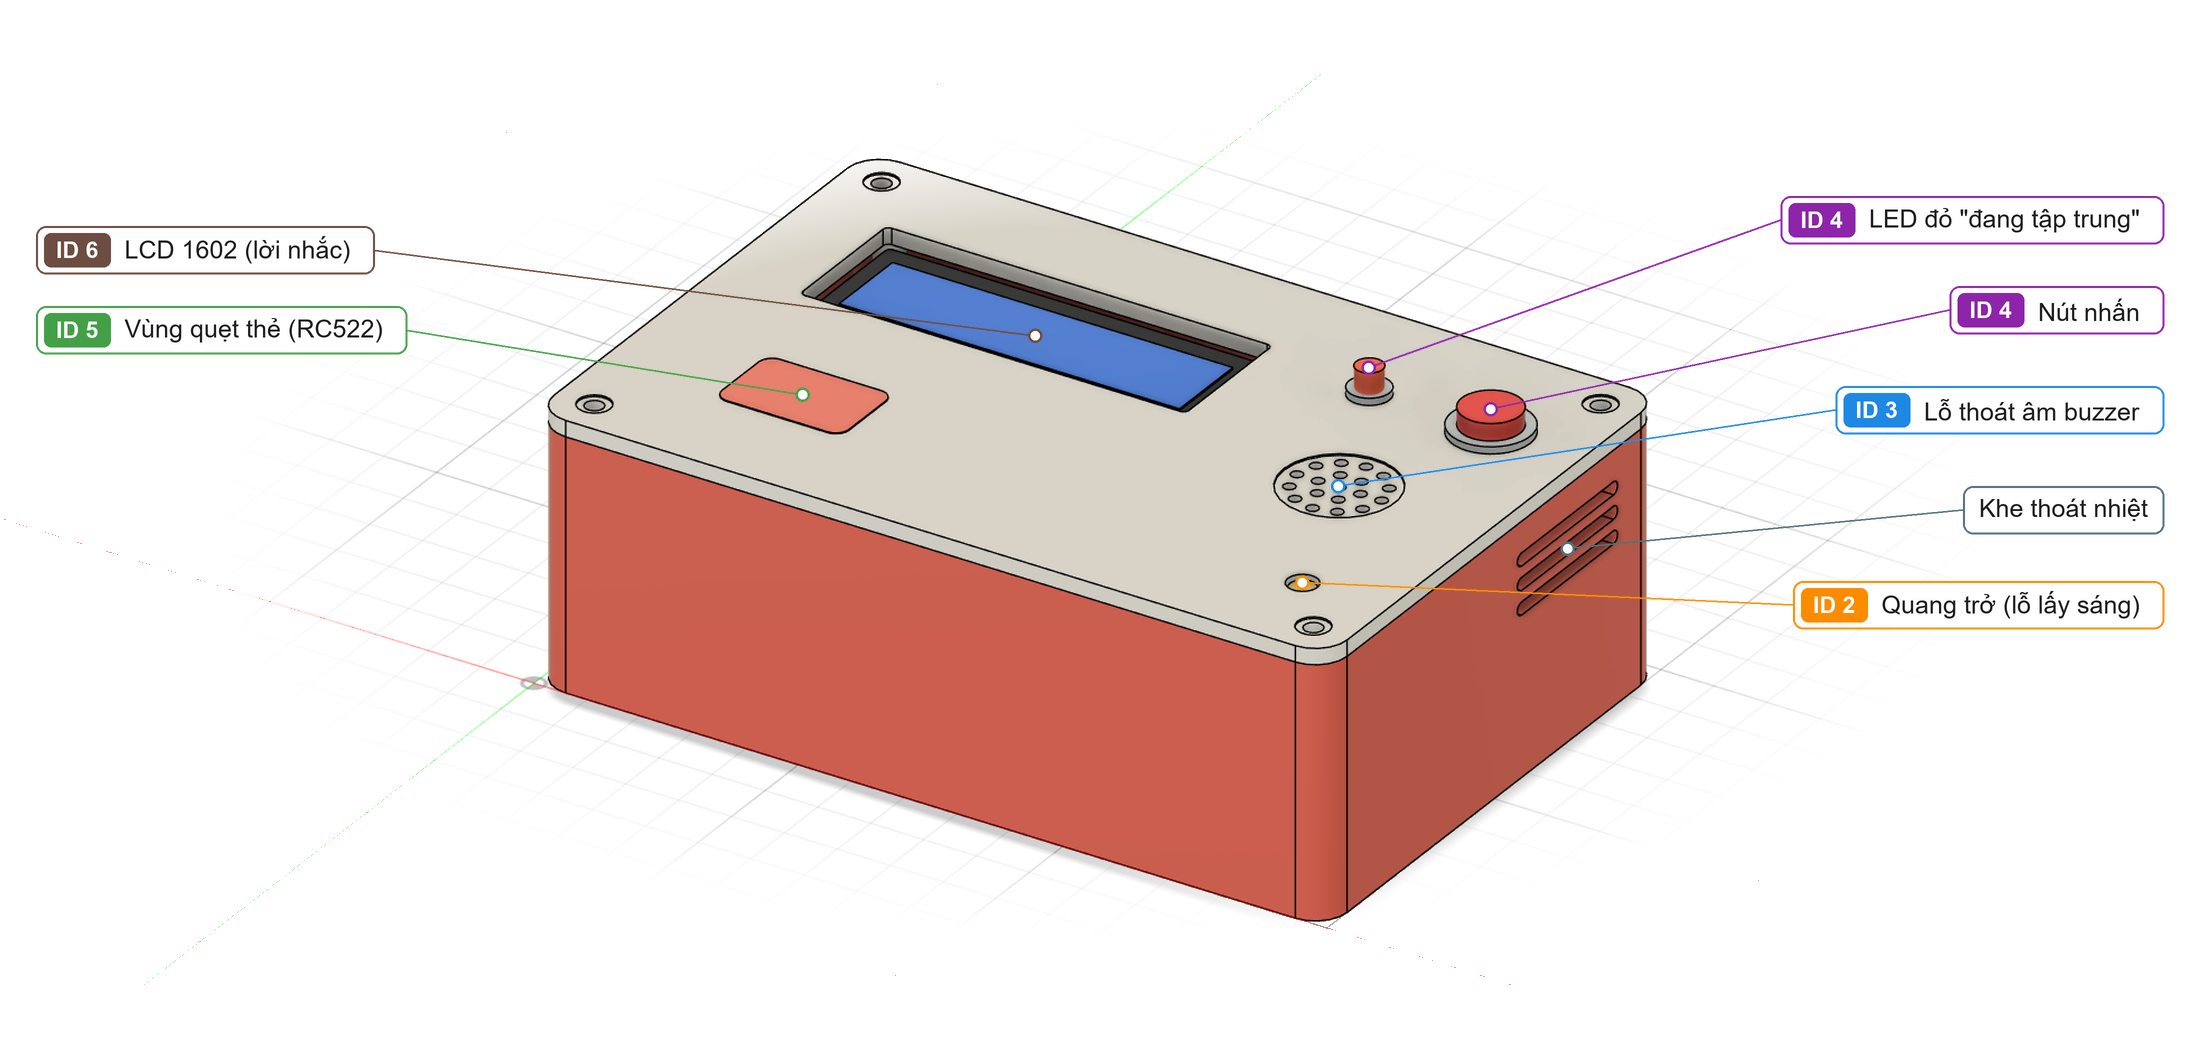
\includegraphics[height=3.0cm, width=\textwidth, keepaspectratio]{assets/design_fusion360/hinh_3d_1_ben_ngoai_truoc.png}
        \caption{Ngoại quan mặt trước (LCD, Nút nhấn, LED, RFID)}
        \label{fig:3d_front}
    \end{subfigure}
    \hfill
    \begin{subfigure}[b]{0.46\textwidth}
        \centering
        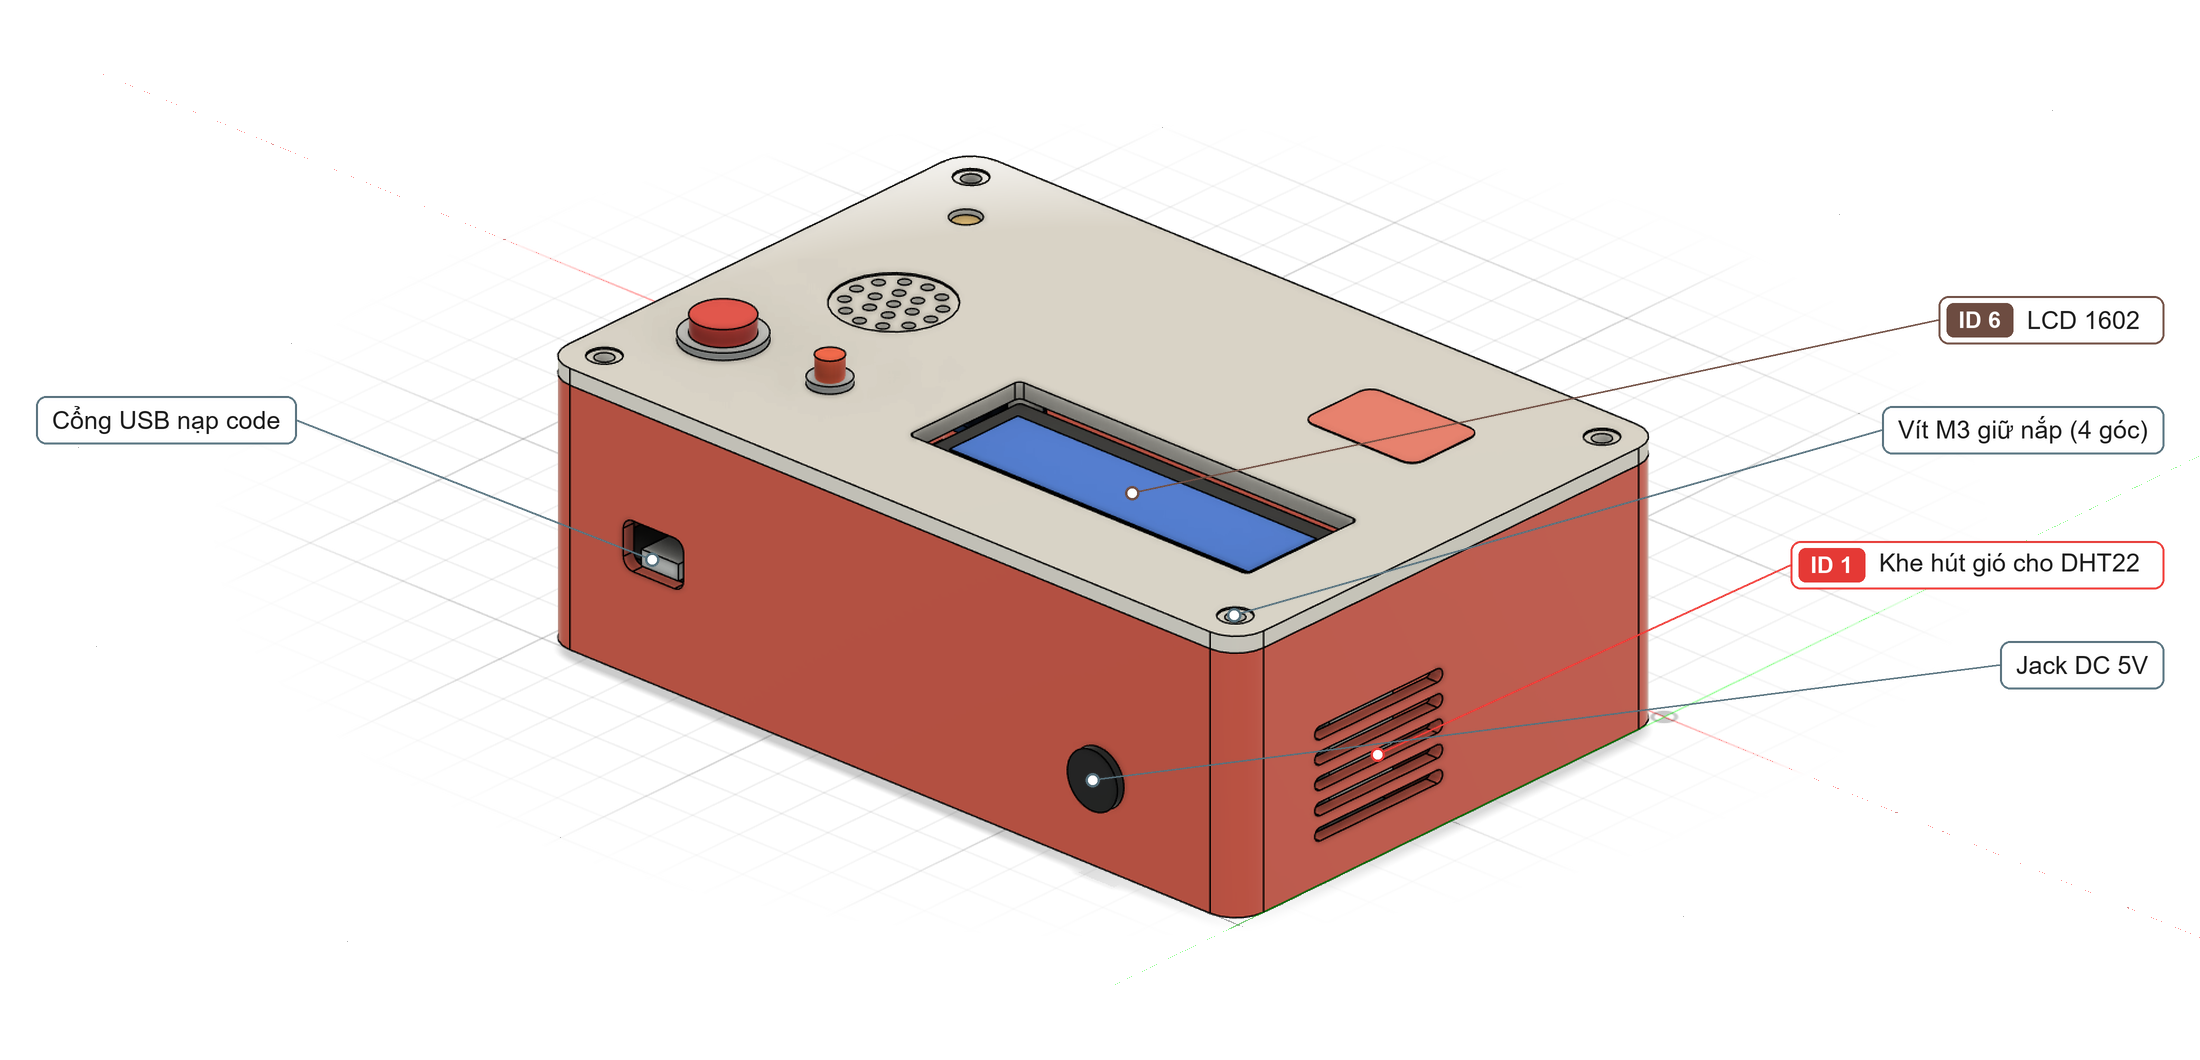
\includegraphics[height=3.0cm, width=\textwidth, keepaspectratio]{assets/design_fusion360/hinh_3d_2_ben_ngoai_sau.png}
        \caption{Ngoại quan mặt sau (Cổng USB, Khe tản nhiệt)}
        \label{fig:3d_back}
    \end{subfigure}
    \par\vspace{0.06cm}
    \begin{subfigure}[b]{0.46\textwidth}
        \centering
        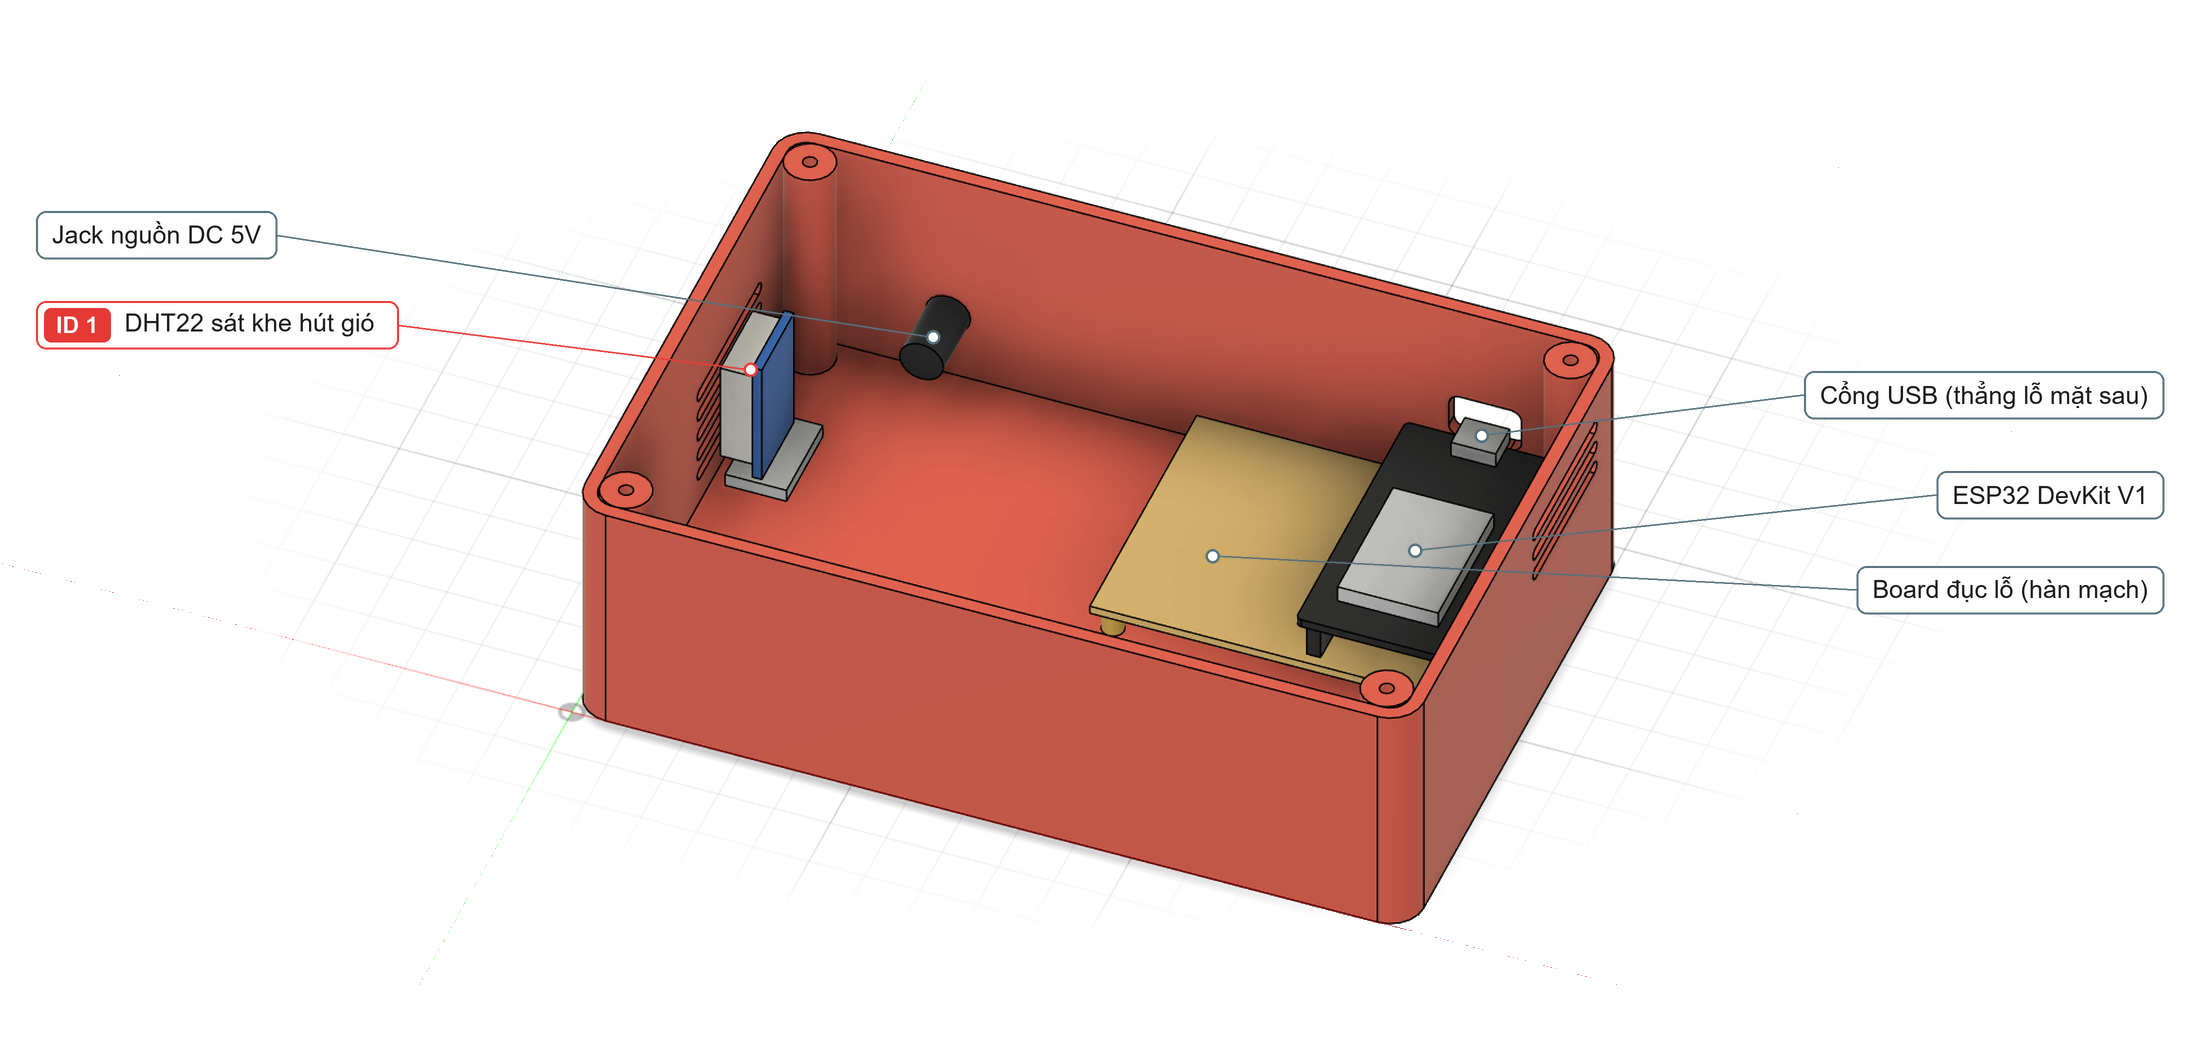
\includegraphics[height=3.0cm, width=\textwidth, keepaspectratio]{assets/design_fusion360/hinh_3d_3_ben_trong_than_hop.png}
        \caption{Bố trí linh kiện bên trong thân hộp}
        \label{fig:3d_inside}
    \end{subfigure}
    \hfill
    \begin{subfigure}[b]{0.46\textwidth}
        \centering
        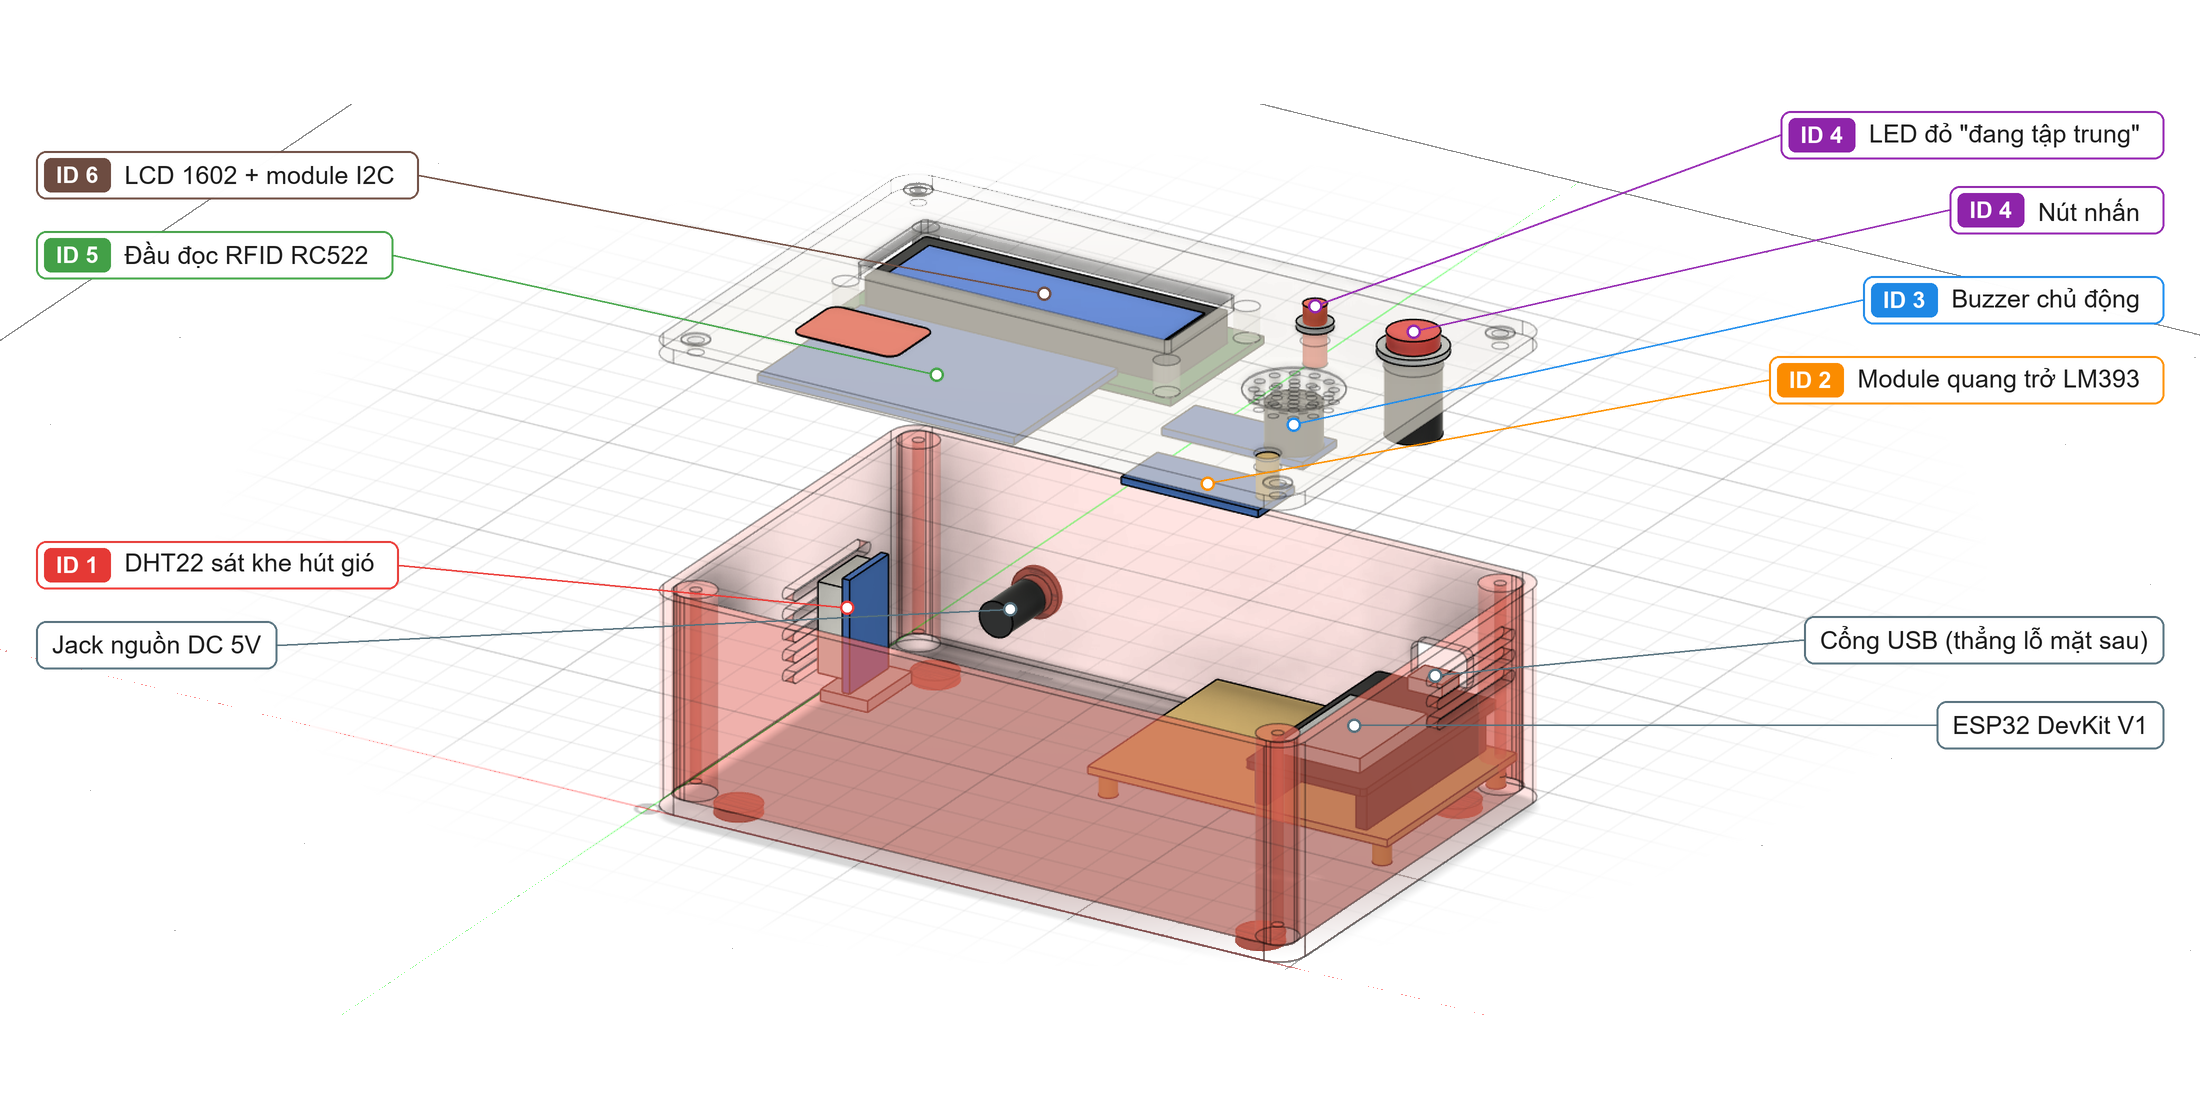
\includegraphics[height=3.0cm, width=\textwidth, keepaspectratio]{assets/design_fusion360/hinh_3d_5_tach_nap.png}
        \caption{Bản vẽ bóc tách nắp và thân (Exploded View)}
        \label{fig:3d_exploded}
    \end{subfigure}
    \vspace{0.06cm}
    \captionof{figure}{Bản vẽ phối cảnh 3D bên ngoài và bên trong vỏ hộp Trạm học tập Pomodoro}
    \label{fig:3d_full}
\end{center}

\clearpage
\subsection{Hình ảnh wireframe cho website quản lý sản phẩm}

Giao diện website quản lý sản phẩm được thiết kế trên nền tảng Node-RED Dashboard phục vụ việc theo dõi và điều khiển trạm học tập. Toàn bộ các vùng chức năng trên bản vẽ wireframe đều được ánh xạ trực tiếp với danh sách các chức năng đã đăng ký ở Mục 1, được tổng hợp chi tiết trong Bảng \ref{tab:map_wireframe_chuc_nang}.

\begin{center}
\scriptsize
\renewcommand{\arraystretch}{0.94}
\begin{tabular}{|c|p{3.8cm}|p{6.6cm}|c|}
\hline
\textbf{STT} & \textbf{Vùng giao diện trên Web} & \textbf{Thành phần hiển thị \& Tác vụ tương tác} & \textbf{ID Chức năng} \\ \hline
1 & Cửa sổ Khí hậu (Climate) & Chỉ số DHT22 ($^\circ\text{C}, \%$), Sparkline 1 giờ, nhãn tiện nghi & \textbf{ID 1} \\ \hline
2 & Cửa sổ Ánh sáng (Light) & Số đo ADC quang trở ($0 - 4095$), nhãn Đủ/Thiếu sáng, thanh đo mức & \textbf{ID 4} \\ \hline
3 & Cửa sổ Hẹn giờ (Timer · Buzzer) & Đồng hồ số đếm ngược, thanh tiến trình, nút Gửi lệnh / Dừng & \textbf{ID 3} \\ \hline
4 & Cửa sổ Lời nhắc LCD 16×2 & Khung nhập văn bản, bộ đếm ký tự, gửi lời nhắc xuống màn hình & \textbf{ID 5} \\ \hline
5 & Cửa sổ Phiên thẻ RFID \& Feedback & Bộ đếm thời gian, mã thẻ UID, cảnh báo Telegram ($>50$p), nút quẹt giả lập, khối phản hồi sau phiên & \textbf{ID 2, ID 6, ID 9, ID 13} \\ \hline
6 & Đèn báo trạng thái tập trung & Biểu tượng hiển thị trạng thái đồng bộ với đèn LED đỏ GPIO26 & \textbf{ID 6} \\ \hline
7 & Cửa sổ Nhật ký & Danh sách sự kiện MQTT thời gian thực, bộ lọc tuần/tháng/năm & \textbf{ID 7} \\ \hline
8 & Đồ thị chuỗi thời gian 24 giờ & Biểu đồ đường kép (Line Chart) nhiệt/ẩm 24h truy vấn từ Supabase & \textbf{ID 7, ID 8} \\ \hline
9 & Khung mô hình AI khuyến nghị & Bảng 3 chỉ số: Thời lượng lý tưởng, Khung giờ vàng, Vi khí hậu & \textbf{ID 13} \\ \hline
10 & Màn hình Cài đặt (Settings) & Cấu hình chu kỳ Pomodoro, nhắc nghỉ Telegram, email tuần, danh sách thẻ & \textbf{ID 9, 10, 12} \\ \hline
11 & Màn hình Đăng nhập \& Đăng ký & Giao diện đăng nhập/tạo tài khoản, hiển thị trạng thái kết nối trạm & \textbf{ID 11} \\ \hline
\end{tabular}
\captionof{table}{Bảng ánh xạ các vùng thiết kế Wireframe Website với ID chức năng}
\label{tab:map_wireframe_chuc_nang}
\end{center}

\subsubsection{Chi tiết các màn hình giao diện và cấu trúc thành phần Node-RED Dashboard}

Hệ thống giao diện được tổ chức theo cấu trúc của Node-RED Dashboard: \textbf{Trang (\texttt{ui\_tab}) $\rightarrow$ Nhóm (\texttt{ui\_group}) $\rightarrow$ Thành phần hiển thị/điều khiển (\texttt{ui\_component})}. Dưới đây là hình ảnh wireframe các màn hình và đặc tả thành phần tương ứng:

\clearpage

\begin{center}
\captionsetup{type=figure}
    \begin{subfigure}[b]{0.48\textwidth}
        \centering
        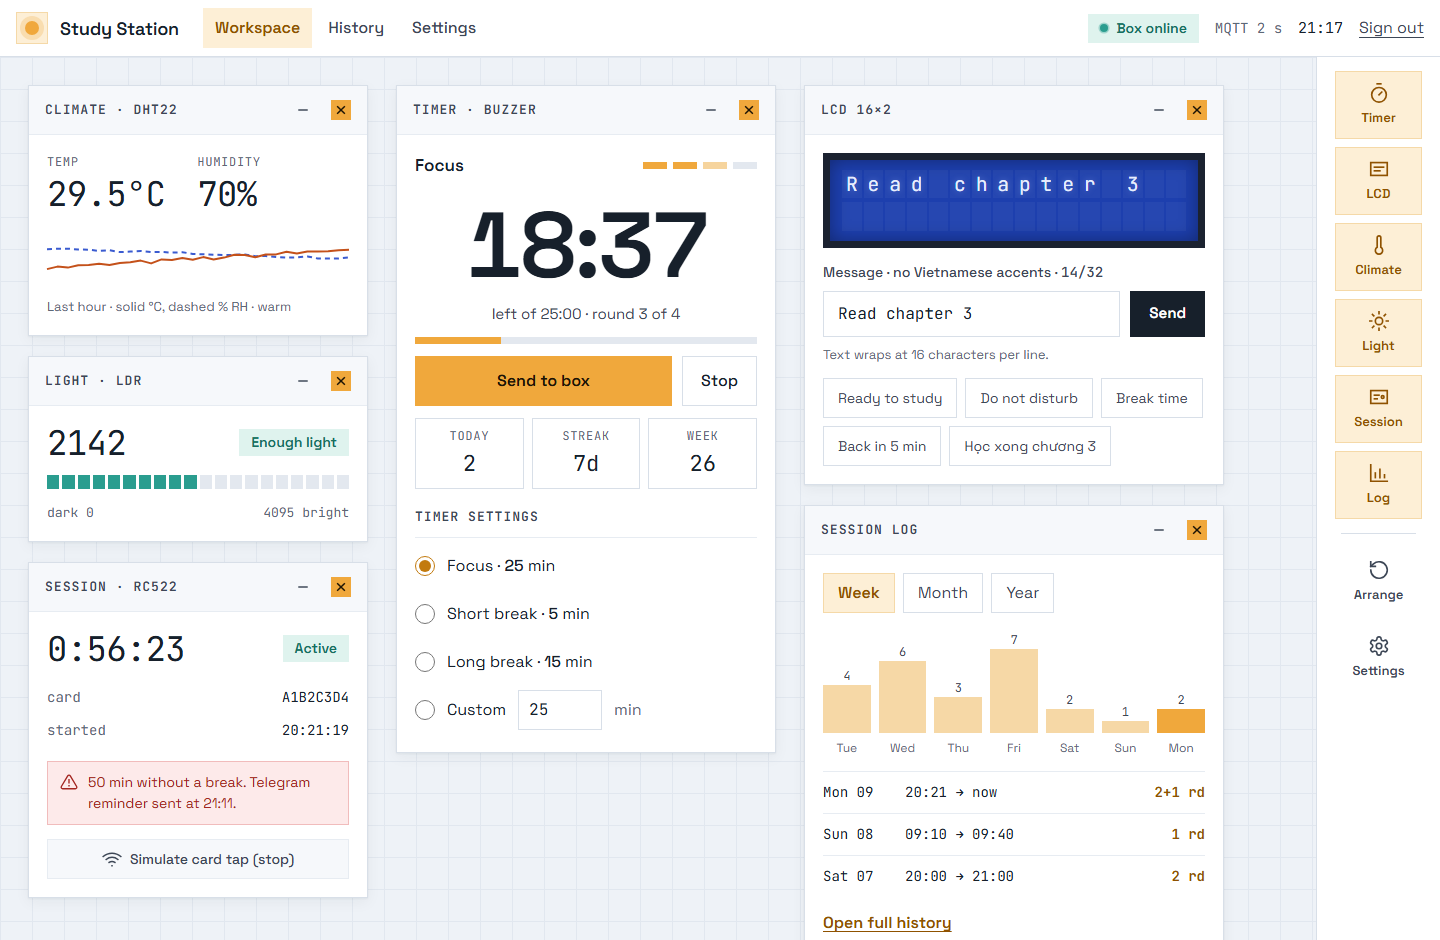
\includegraphics[height=3.0cm, width=\textwidth, keepaspectratio]{assets/wireframes/03-workspace-desktop.png}
        \caption{Bàn làm việc Workspace Desktop (6 cửa sổ điều khiển)}
        \label{fig:wf_workspace}
    \end{subfigure}
    \hfill
    \begin{subfigure}[b]{0.48\textwidth}
        \centering
        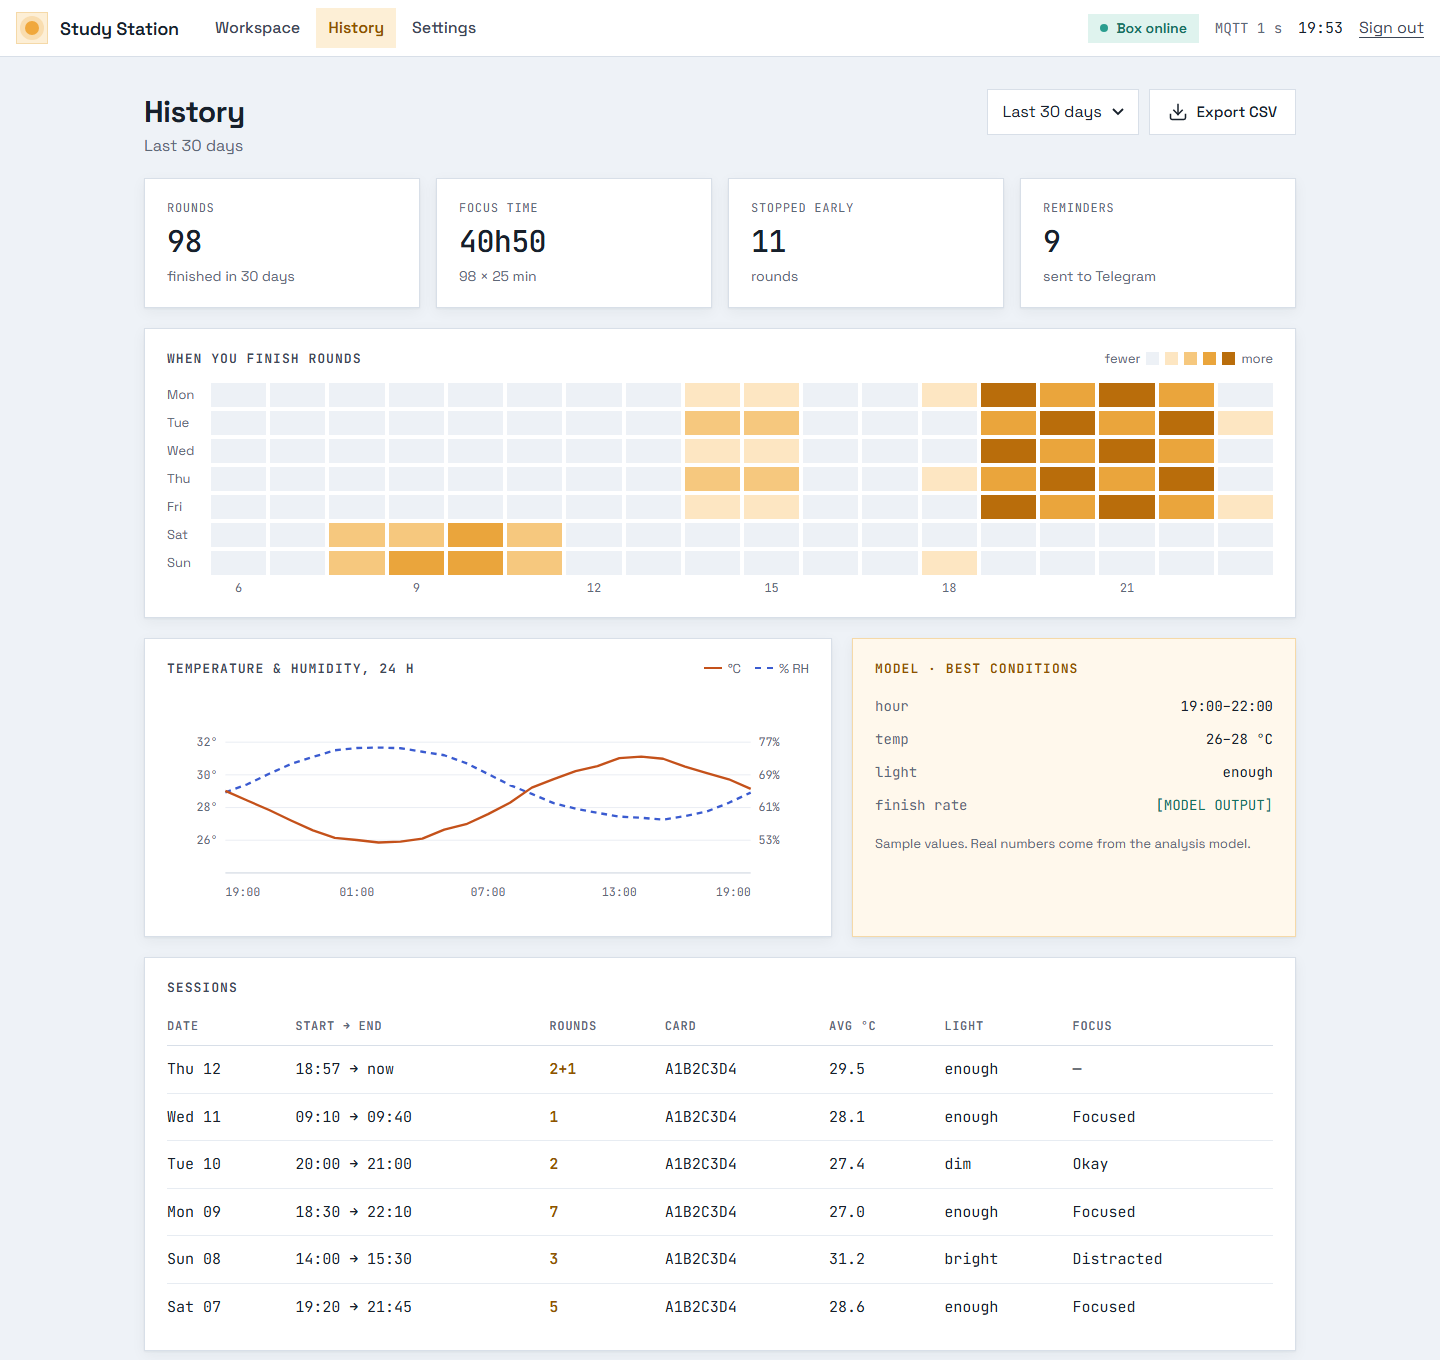
\includegraphics[height=3.0cm, width=\textwidth, keepaspectratio]{assets/wireframes/04-history-desktop.png}
        \caption{Trang Lịch sử, biểu đồ thời gian và khối khuyến nghị}
        \label{fig:wf_history}
    \end{subfigure}
    \vspace{0.04cm}
    \captionof{figure}{Giao diện Bàn làm việc Workspace và Lịch sử phân tích dữ liệu trên Desktop (ID 1--8, 13)}
    \label{fig:wf_desktop_main}
\end{center}

\textbf{Cấu trúc thành phần Node-RED Dashboard cho Bàn làm việc và Lịch sử (Hình \ref{fig:wf_desktop_main}):}
\begin{itemize}[leftmargin=0.6cm, noitemsep, topsep=1pt]
    \sloppy
    \item \textbf{Trang Bàn làm việc (\texttt{ui\_tab}: \texttt{tab\_workspace}):} \texttt{ui\_template} (Thanh điều hướng đỉnh và khay tiện ích); \texttt{ui\_group} (\texttt{win\_timer} -- ID 3: \texttt{ui\_template} đếm ngược số lớn kèm thanh tiến trình, \texttt{ui\_button} Bắt đầu/Dừng, \texttt{ui\_dropdown} tùy chọn 25p/5p/15p hoặc tùy chỉnh); \texttt{ui\_group} (\texttt{win\_lcd} -- ID 5: \texttt{ui\_template} giả lập LCD 1602, \texttt{ui\_text\_input} nhập lời nhắc, \texttt{ui\_button} gửi lệnh); \texttt{ui\_group} (\texttt{win\_climate} -- ID 1: \texttt{ui\_text} số đo nhiệt độ/độ ẩm DHT22, \texttt{ui\_chart} biểu đồ Sparkline 1h); \texttt{ui\_group} (\texttt{win\_light} -- ID 4: \texttt{ui\_text} ADC quang trở $0-4095$, \texttt{ui\_template} thanh đo sáng); \texttt{ui\_group} (\texttt{win\_session} -- ID 2, 6, 9: \texttt{ui\_text} đếm phiên/mã thẻ UID, LED đỏ GPIO26, \texttt{ui\_template} khung cảnh báo Telegram $>50$p, \texttt{ui\_button} quẹt thẻ thử nghiệm); \texttt{ui\_group} (\texttt{win\_log} -- ID 7: \texttt{ui\_button} lọc dữ liệu tuần/tháng, danh sách sự kiện MQTT).
    \item \textbf{Trang Lịch sử \& Phân tích (\texttt{ui\_tab}: \texttt{tab\_history}):} \texttt{ui\_group} (4 widget \texttt{ui\_text} tóm tắt 30 ngày gồm Tổng phiên, Giờ tập trung, Phiên hủy, Cảnh báo Telegram); \texttt{ui\_group} (\texttt{grp\_hist\_heatmap}: \texttt{ui\_template} ma trận chuyên cần theo ngày và giờ); \texttt{ui\_group} (\texttt{grp\_hist\_chart} -- ID 7, 8: \texttt{ui\_chart} biểu đồ đường kép 24h chuỗi thời gian nhiệt độ $^\circ\text{C}$ và độ ẩm $\%$ từ Supabase); \texttt{ui\_group} (\texttt{grp\_hist\_model} -- ID 13: \texttt{ui\_template} bảng hiển thị thông số khuyến nghị từ mô hình phân tích); \texttt{ui\_group} (bảng danh sách chi tiết các phiên học gồm Ngày, Giờ, Mã thẻ, Vi khí hậu, đánh giá tập trung).
\end{itemize}

\clearpage

\begin{center}
\captionsetup{type=figure}
    \begin{subfigure}[b]{0.31\textwidth}
        \centering
        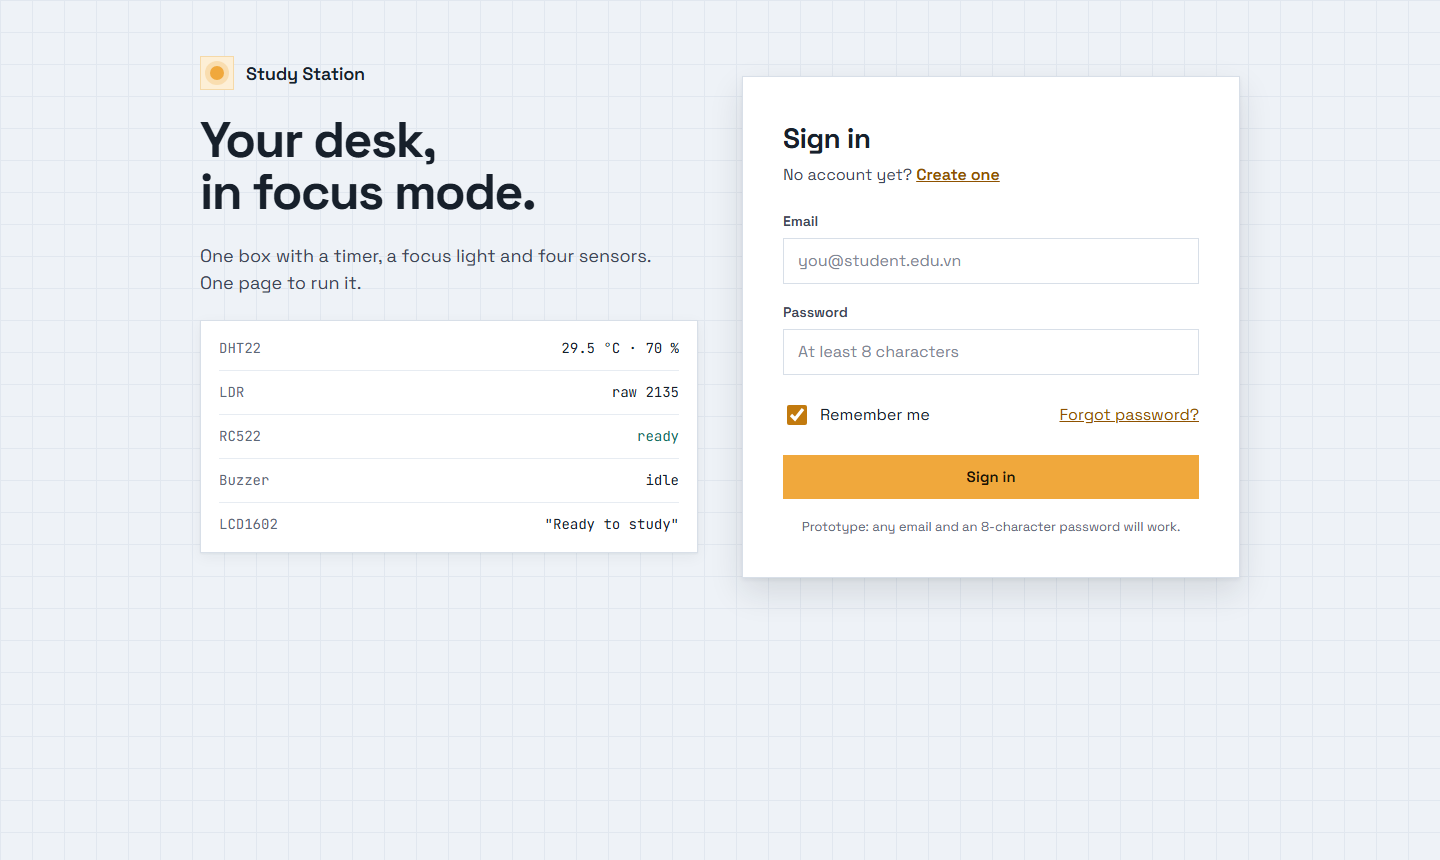
\includegraphics[height=2.8cm, width=\textwidth, keepaspectratio]{assets/wireframes/01-sign-in-desktop.png}
        \caption{Đăng nhập (Sign in)}
        \label{fig:wf_signin}
    \end{subfigure}
    \hfill
    \begin{subfigure}[b]{0.31\textwidth}
        \centering
        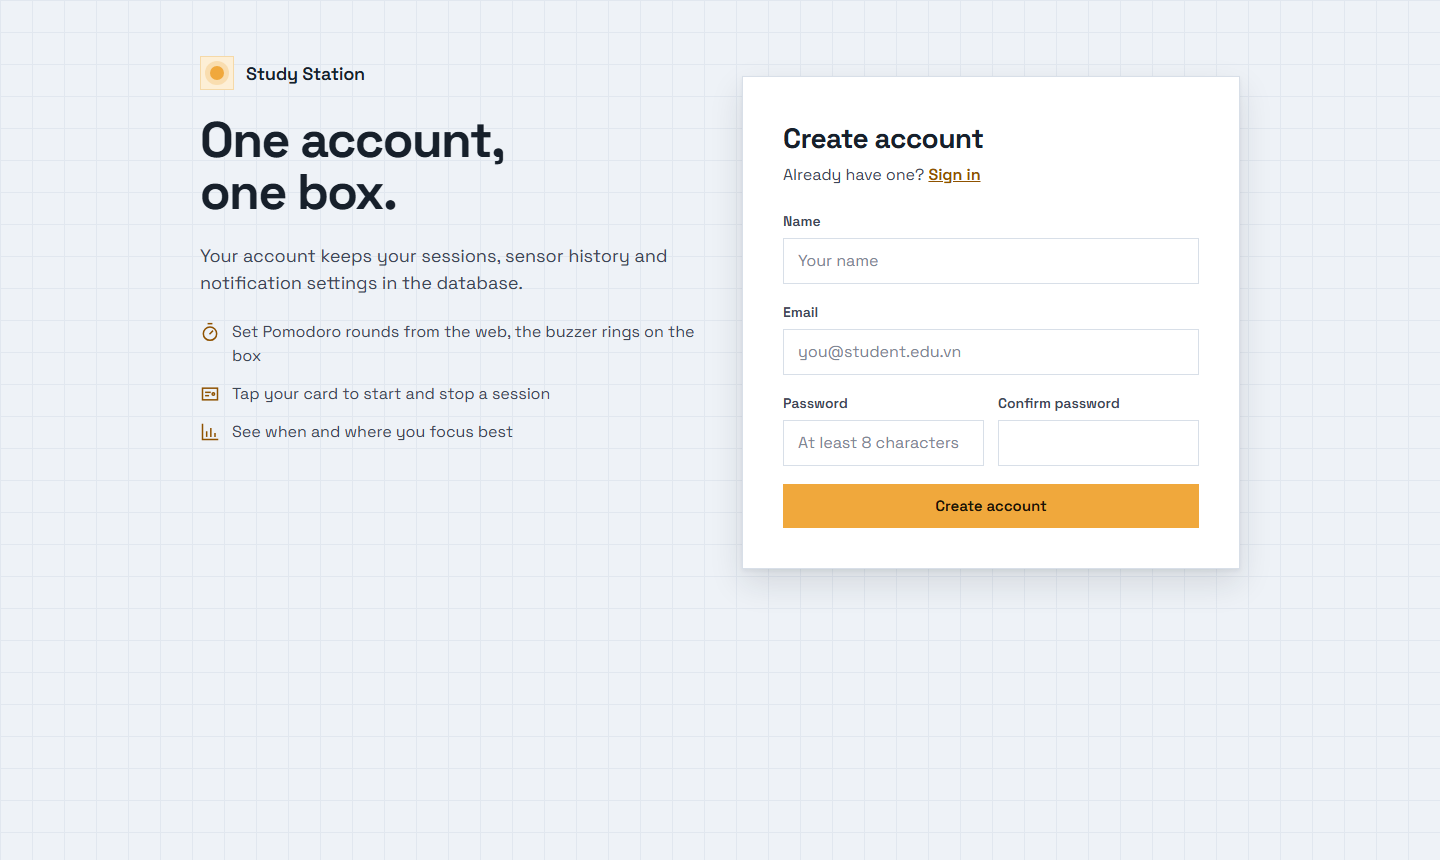
\includegraphics[height=2.8cm, width=\textwidth, keepaspectratio]{assets/wireframes/02-register-desktop.png}
        \caption{Đăng ký (Register)}
        \label{fig:wf_register}
    \end{subfigure}
    \hfill
    \begin{subfigure}[b]{0.31\textwidth}
        \centering
        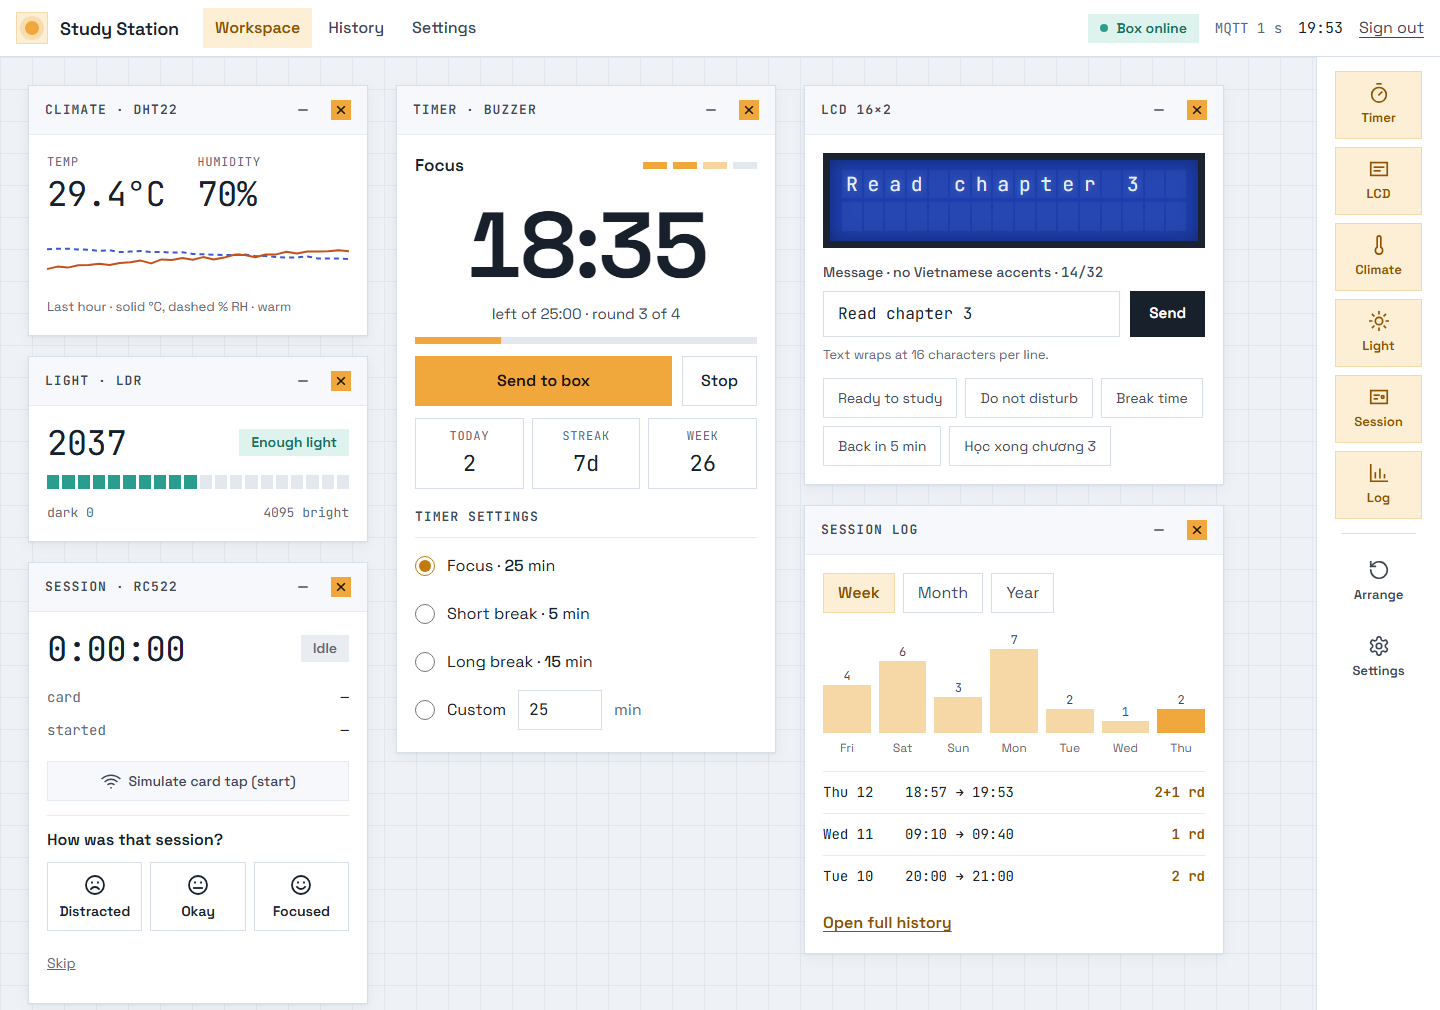
\includegraphics[height=2.8cm, width=\textwidth, keepaspectratio]{assets/wireframes/14-rating-desktop.png}
        \caption{Đánh giá sau phiên}
        \label{fig:wf_rating}
    \end{subfigure}
    \vspace{0.04cm}
    \captionof{figure}{Giao diện Xác thực người dùng (ID 11) và Khối đánh giá sau phiên học (ID 13)}
    \label{fig:wf_auth_rating}
\end{center}

\textbf{Cấu trúc thành phần Node-RED Dashboard cho Xác thực và Đánh giá sau phiên (Hình \ref{fig:wf_auth_rating}):}
\begin{itemize}[leftmargin=0.8cm, noitemsep, topsep=1pt]
    \sloppy
    \item \textbf{Trang Xác thực (\texttt{ui\_tab}: \texttt{tab\_auth} -- ID 11):} \texttt{ui\_group} (hiển thị trạng thái kết nối các module DHT22, LM393, RC522, Buzzer, LCD); \texttt{ui\_group} (\texttt{ui\_text\_input} Họ tên, Email, Mật khẩu $\ge 8$ ký tự; \texttt{ui\_switch} ghi nhớ đăng nhập; \texttt{ui\_button} kích hoạt hàm băm mật mã bcrypt).
    \item \textbf{Khối Đánh giá sau phiên (\texttt{ui\_group}: \texttt{win\_session\_rating} -- ID 13):} \texttt{ui\_template} câu hỏi xác nhận mức độ tập trung sau khi kết thúc phiên; 3 nút \texttt{ui\_button} ghi nhận điểm phản hồi vào Supabase: \textbf{Distracted} ($S_f = 0.0$), \textbf{Okay} ($S_f = 0.5$), \textbf{Focused} ($S_f = 1.0$); nút bỏ qua và thông báo hoàn tác.
\end{itemize}

\vspace{0.1cm}

\begin{center}
\captionsetup{type=figure}
    \begin{subfigure}[b]{0.45\textwidth}
        \centering
        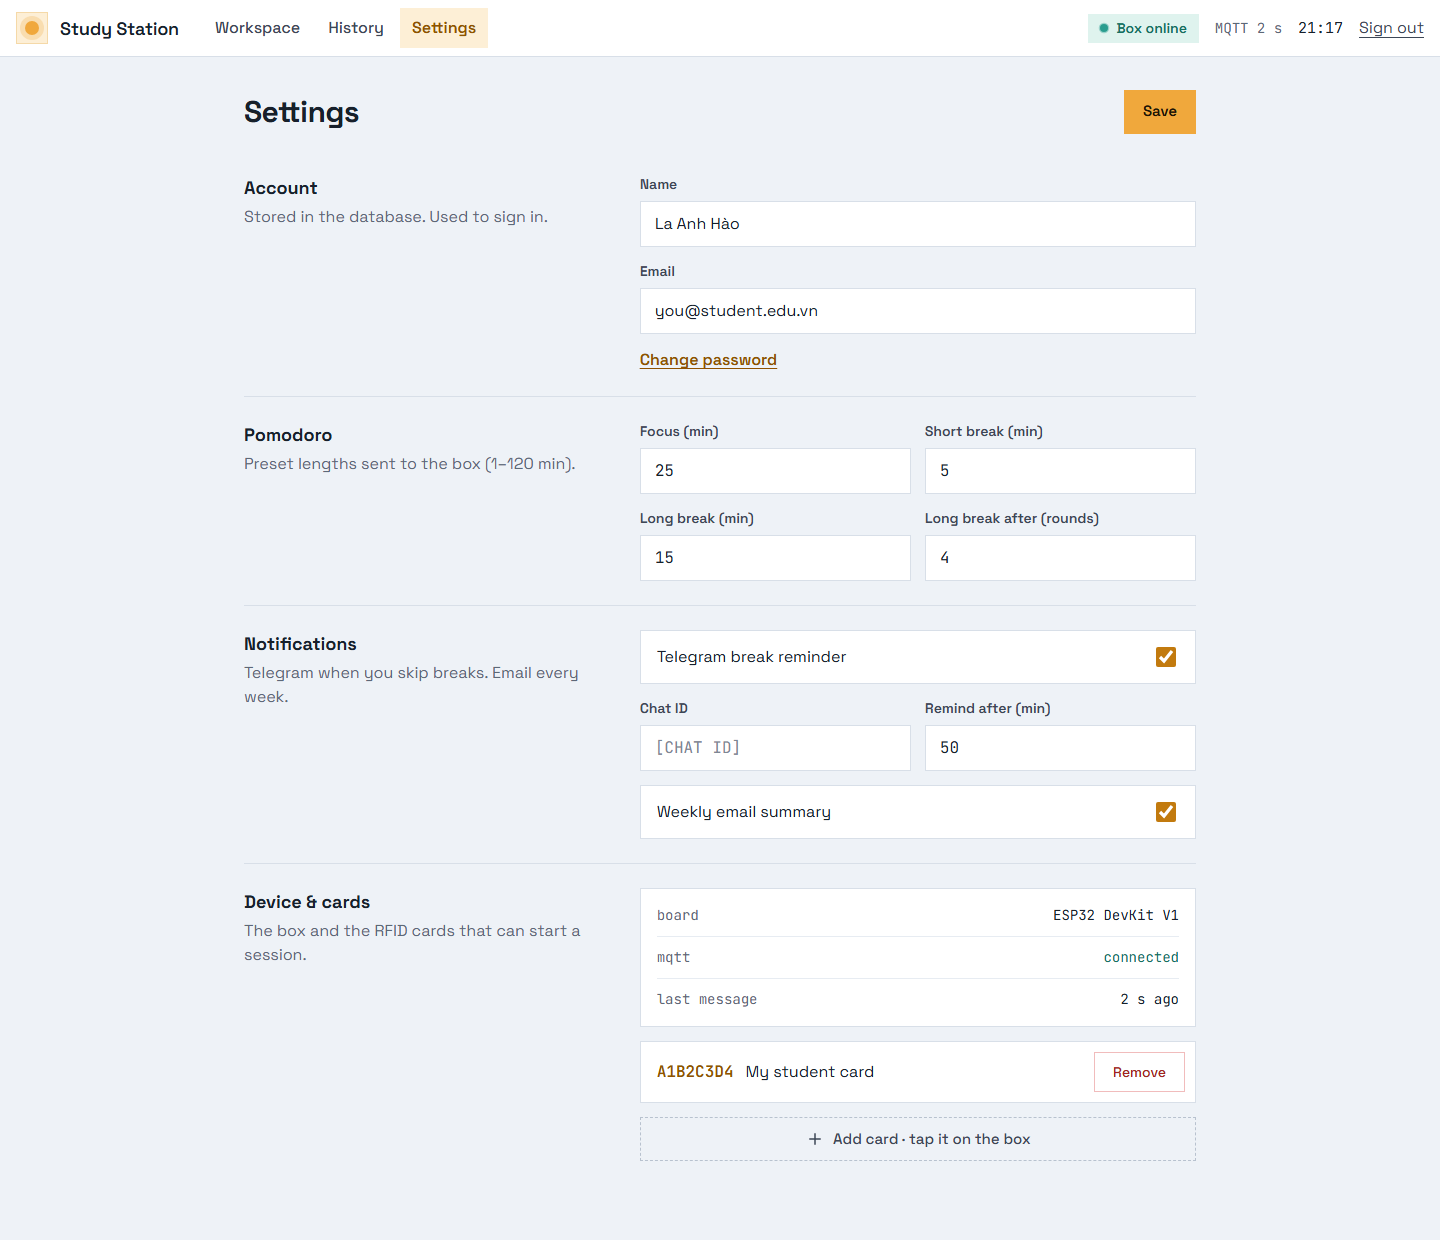
\includegraphics[height=2.8cm, width=\linewidth, keepaspectratio]{assets/wireframes/05-settings-desktop.png}
        \caption{Trang Cài đặt hệ thống (Desktop)}
        \label{fig:wf_settings}
    \end{subfigure}
    \hfill
    \begin{subfigure}[b]{0.52\textwidth}
        \centering
        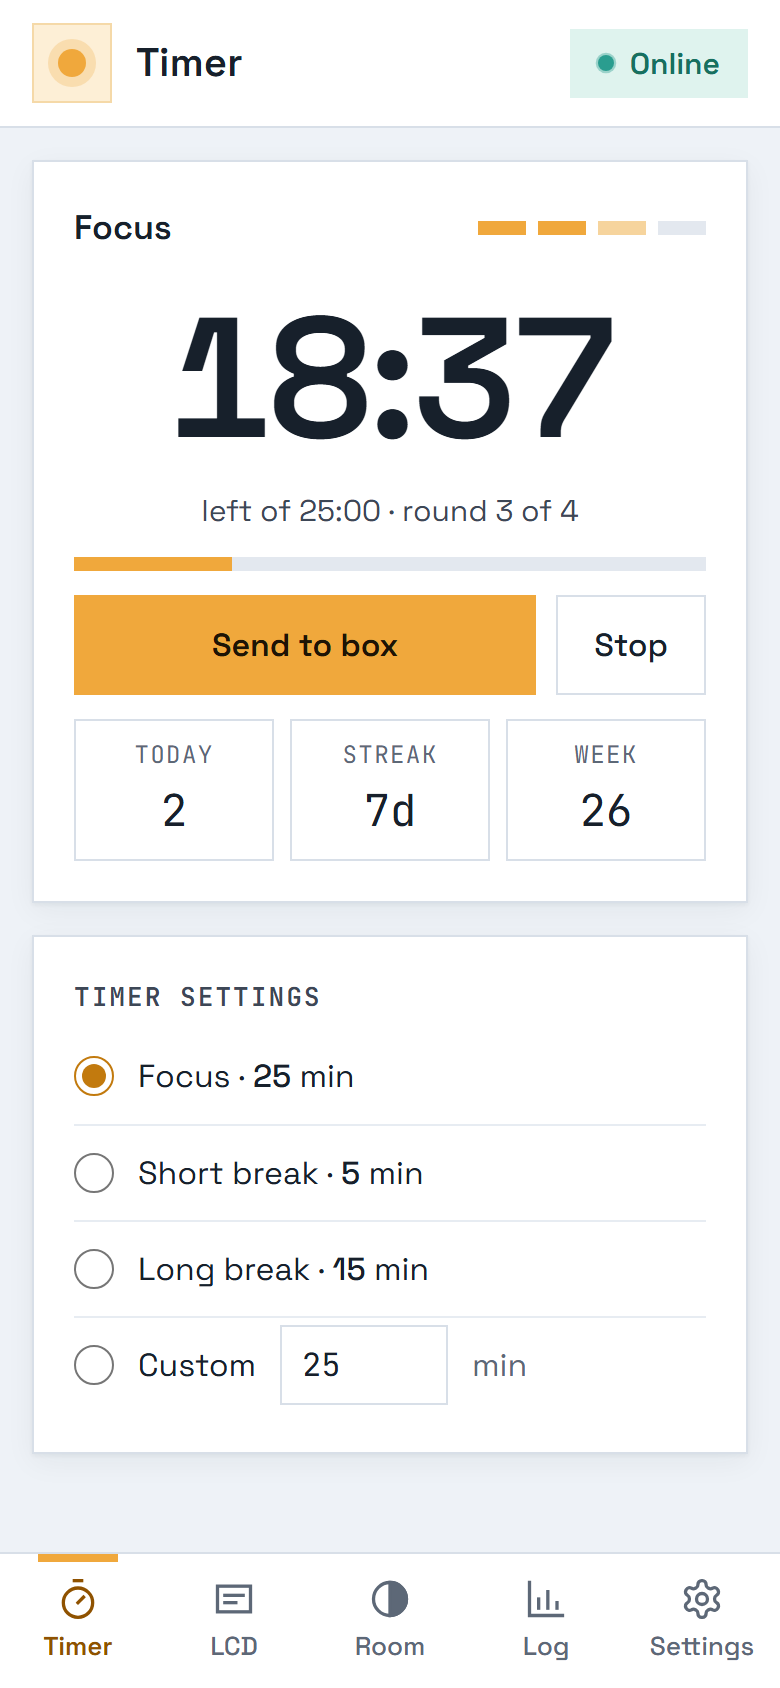
\includegraphics[height=2.8cm, width=0.235\linewidth, keepaspectratio]{assets/wireframes/08-workspace-mobile-timer.png}\hfill
        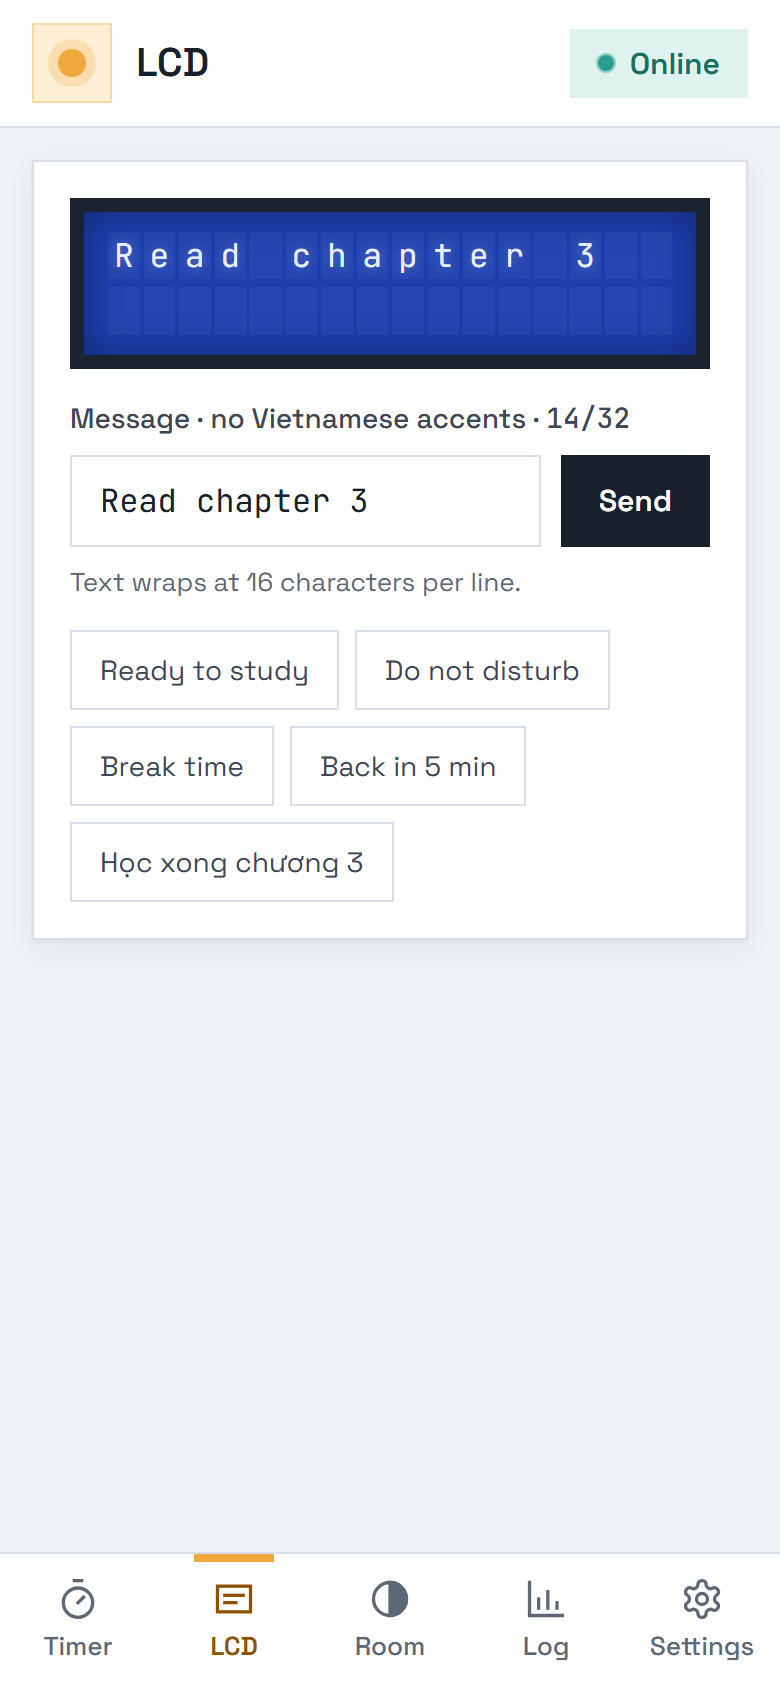
\includegraphics[height=2.8cm, width=0.235\linewidth, keepaspectratio]{assets/wireframes/09-workspace-mobile-lcd.png}\hfill
        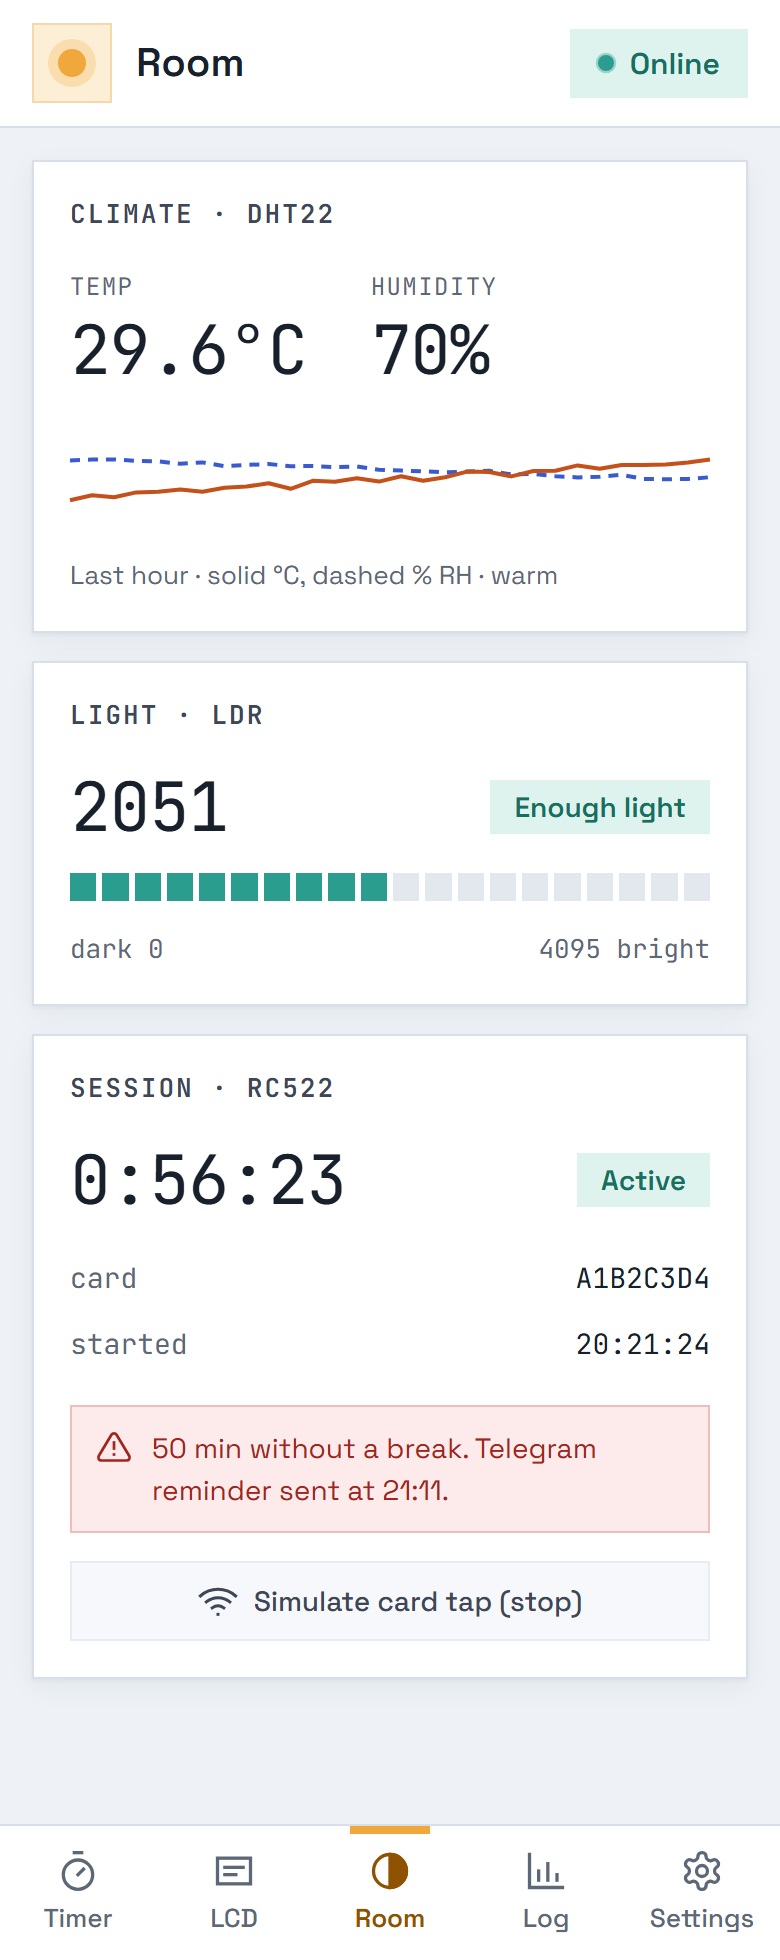
\includegraphics[height=2.8cm, width=0.235\linewidth, keepaspectratio]{assets/wireframes/10-workspace-mobile-room.png}\hfill
        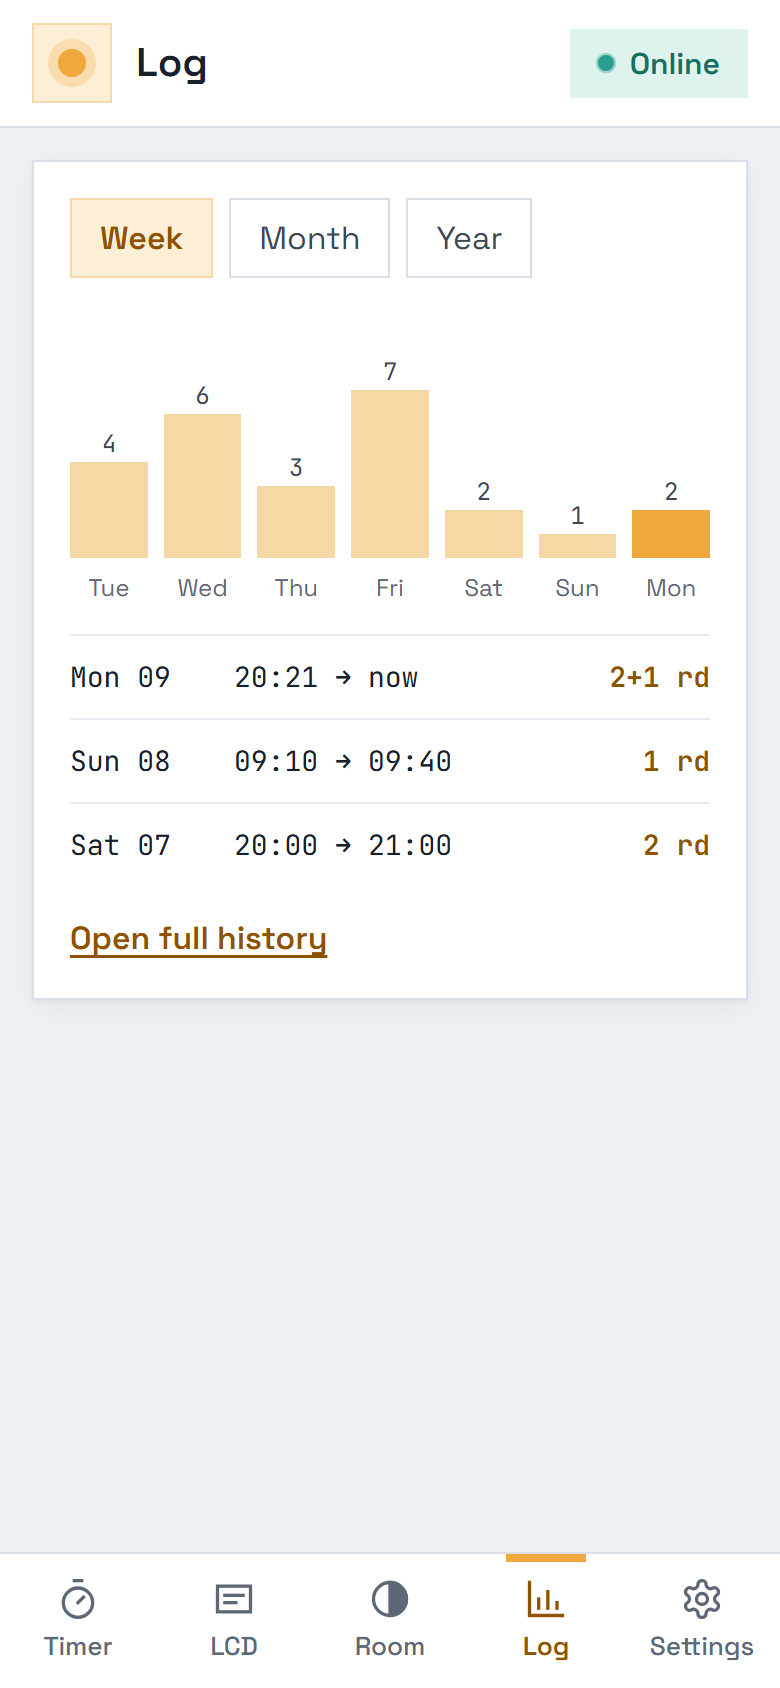
\includegraphics[height=2.8cm, width=0.235\linewidth, keepaspectratio]{assets/wireframes/11-workspace-mobile-log.png}
        \caption{Giao diện Mobile Web App (4 Tab chạm cạnh đáy)}
        \label{fig:wf_mobile}
    \end{subfigure}
    \vspace{0.04cm}
    \captionof{figure}{Giao diện Cài đặt hệ thống (ID 9, 10, 12) và Giao diện thiết bị di động (Mobile Web App)}
    \label{fig:wf_settings_mobile}
\end{center}

\textbf{Cấu trúc thành phần Node-RED Dashboard cho Cài đặt và Ứng dụng di động (Hình \ref{fig:wf_settings_mobile}):}
\begin{itemize}[leftmargin=0.8cm, noitemsep, topsep=1pt]
    \sloppy
    \item \textbf{Trang Cài đặt (\texttt{ui\_tab}: \texttt{tab\_settings} -- ID 3, 9, 10, 12):} \texttt{ui\_group} (\texttt{grp\_set\_pomodoro}: \texttt{ui\_numeric} cài đặt thời gian học $1-120\text{p}$, nghỉ ngắn $1-120\text{p}$, nghỉ dài $1-120\text{p}$, chu kỳ lặp $1-12$ vòng); \texttt{ui\_group} (\texttt{grp\_set\_alerts}: \texttt{ui\_switch} bật Telegram, \texttt{ui\_text\_input} Chat ID, \texttt{ui\_numeric} thời lượng $10-240\text{p}$; \texttt{ui\_switch} bật báo cáo email tuần Gmail SMTP); \texttt{ui\_group} (\texttt{grp\_set\_devices}: \texttt{ui\_text} trạng thái MQTT, \texttt{ui\_template} danh sách thẻ RFID, \texttt{ui\_button} thêm/xóa thẻ).
    \item \textbf{Giao diện Mobile Web App ($\le 760\text{ px}$):} Bố cục 1 cột cuộn; thanh điều hướng cố định cạnh đáy gồm 5 tab chuyển màn hình: \textit{Timer} (Đếm ngược), \textit{LCD} (Lời nhắc), \textit{Room} (Khí hậu, Quang trở, Phiên RFID), \textit{Log} (Nhật ký), và \textit{Settings} (Cài đặt).
\end{itemize}

\clearpage
\subsection{Sơ đồ truyền và nhận dữ liệu giữa các thành phần trong hệ thống}

Toàn bộ các luồng xử lý và đường truyền nhận dữ liệu của 13 chức năng được gộp chung vào một sơ đồ duy nhất tại Hình \ref{fig:so_do_hop_nhat_toan_he_thong}. Sơ đồ mô tả chi tiết đường truyền dữ liệu giữa các cảm biến/linh kiện ngoại vi, vi điều khiển ESP32, máy chủ MQTT Mosquitto, hệ thống điều phối Node-RED, cơ sở dữ liệu Supabase Cloud và các dịch vụ cảnh báo (Telegram Bot, Gmail SMTP). Ba luồng xử lý được phân biệt bằng 3 kiểu đường nét tương ứng với phân công công việc của từng thành viên:
\begin{itemize}[leftmargin=1.2cm, noitemsep, topsep=2pt]
    \item \textbf{Đường nét liền [L1] (Trần Nguyễn Tuấn Minh phụ trách):} Luồng thu thập vi khí hậu và phân tích điều kiện tối ưu (ID 1, 7, 8, 13).
    \item \textbf{Đường nét đứt [L2] (Nguyễn Quốc Dương phụ trách):} Luồng giám sát ánh sáng, điểm danh RFID, đèn báo bận và cảnh báo (ID 2, 4, 6, 9, 10).
    \item \textbf{Đường nét chấm gạch [L3] (La Anh Hào phụ trách):} Luồng hẹn giờ Pomodoro, còi báo, lời nhắc LCD, xác thực bảo mật và SoftAP Wi-Fi (ID 3, 5, 11, 12).
\end{itemize}

\begin{center}
\captionsetup{type=figure}
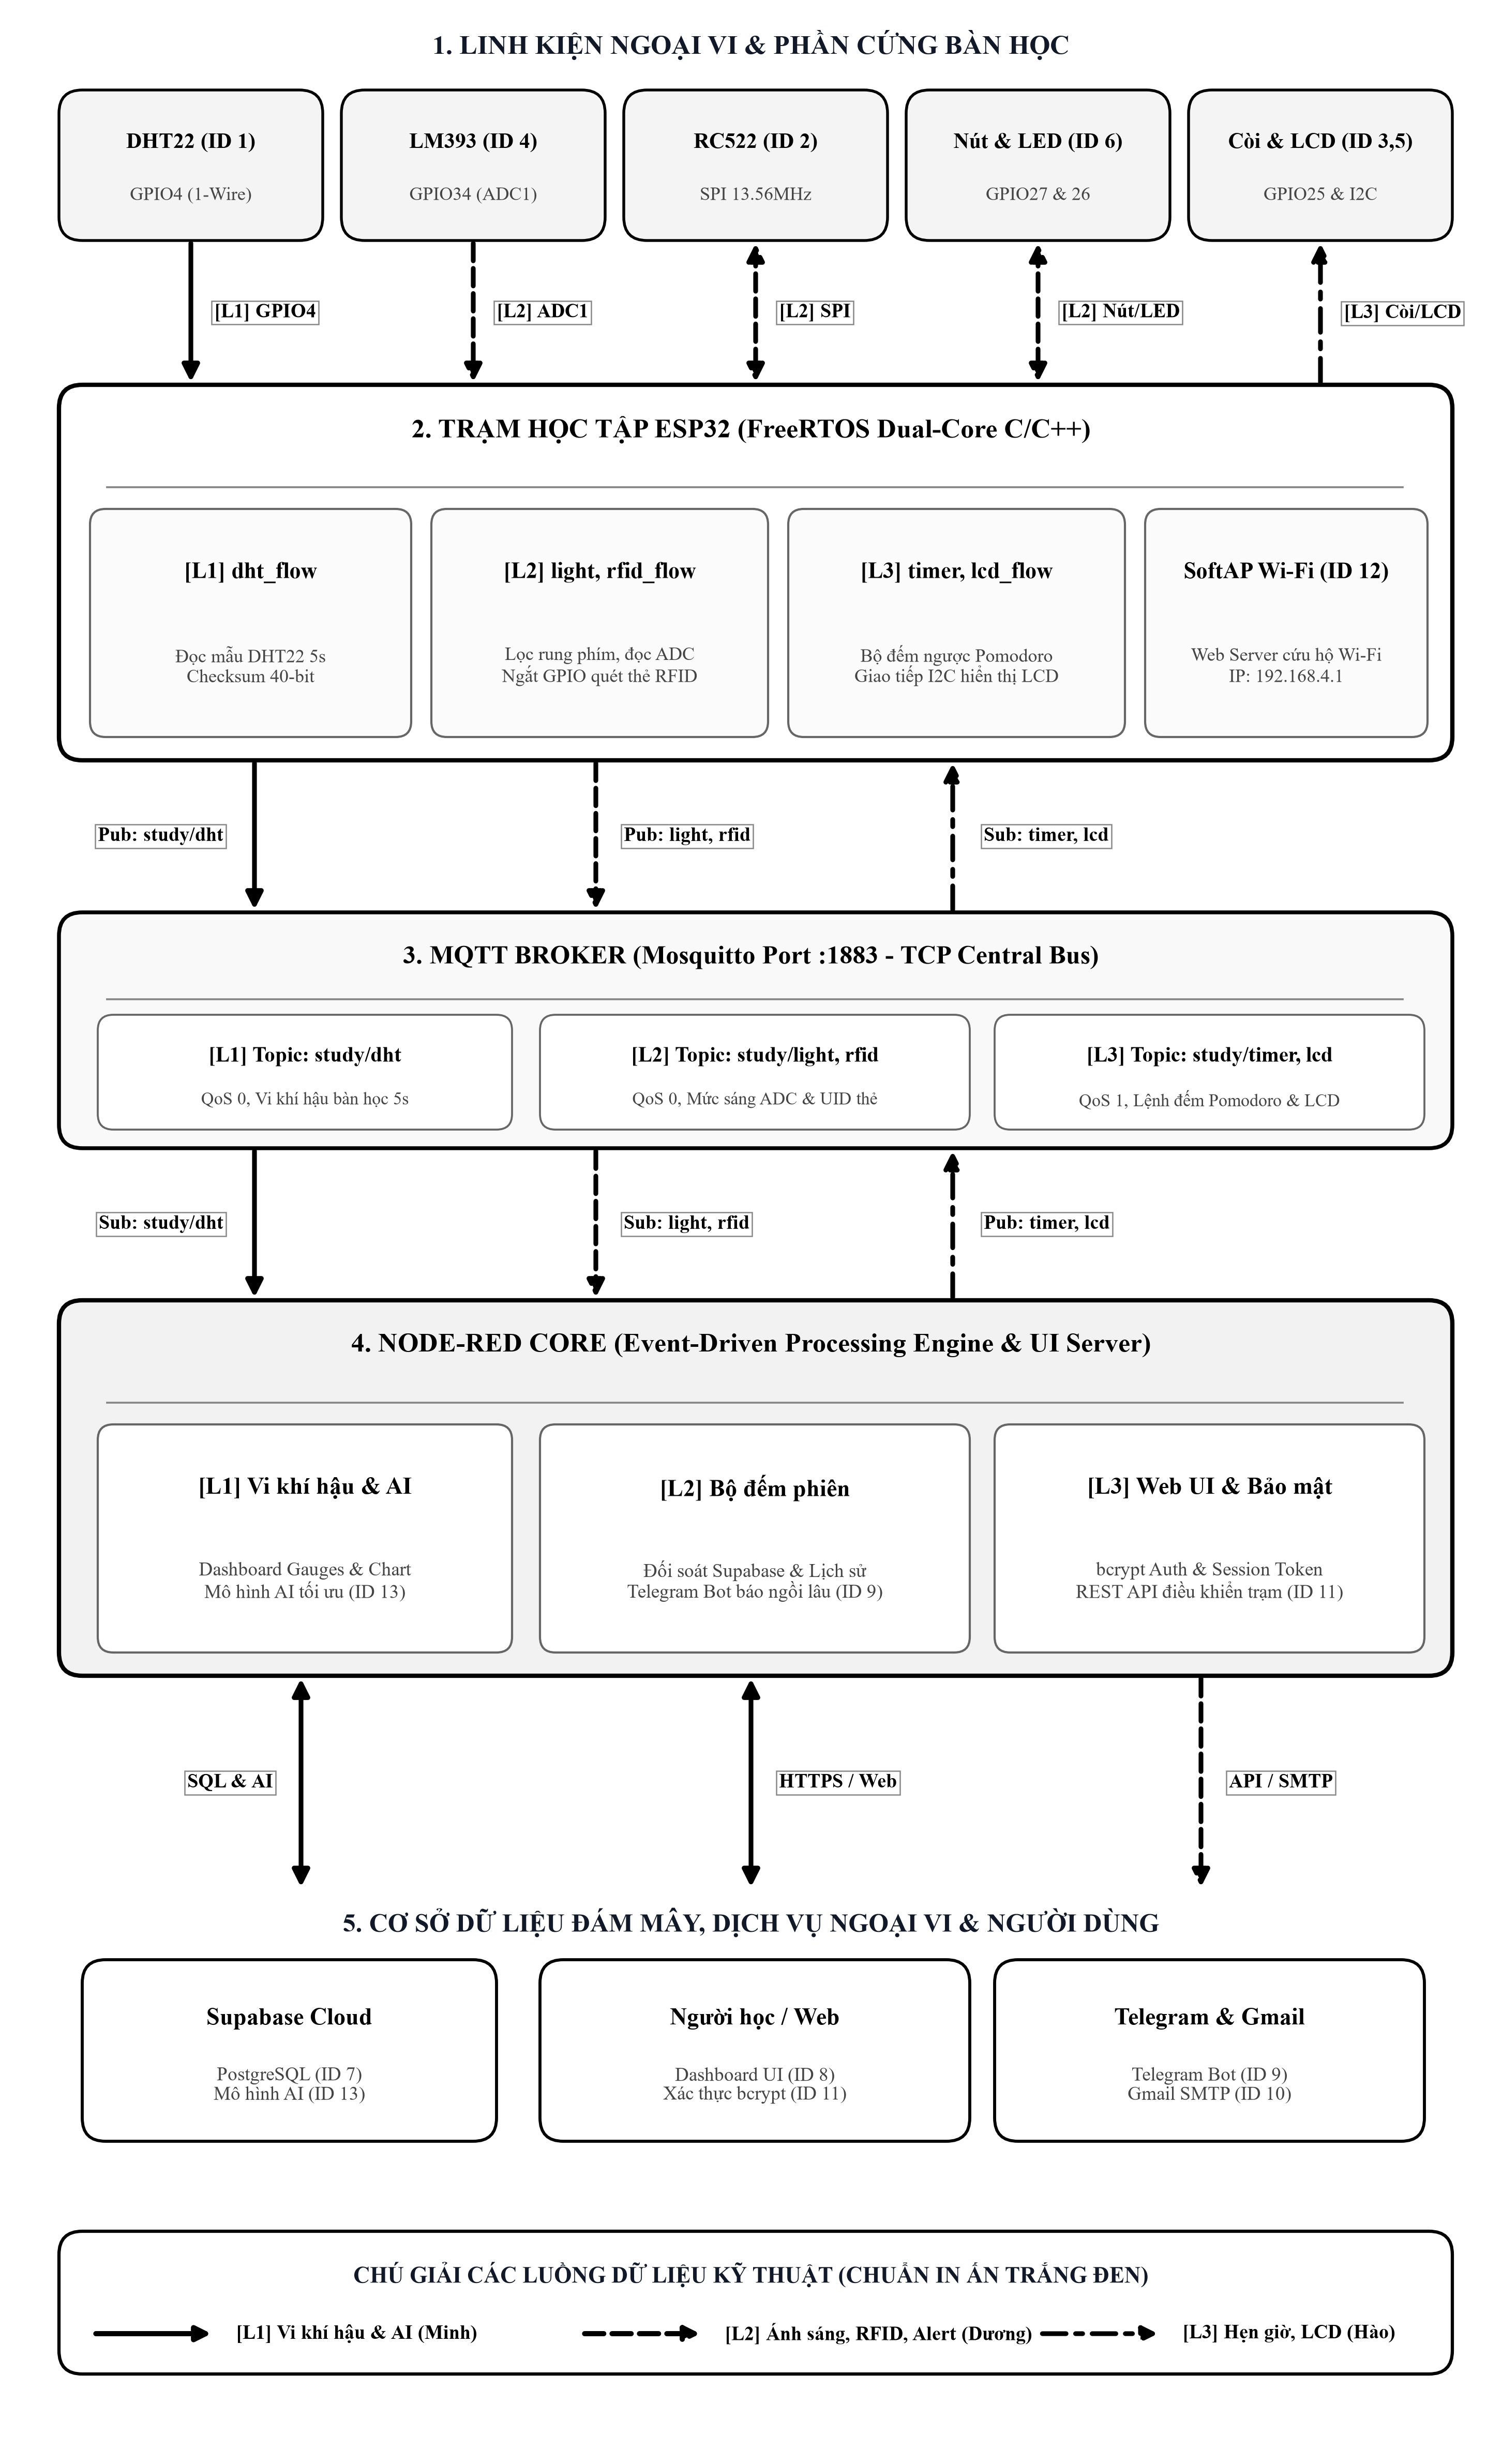
\includegraphics[height=19.5cm, width=\textwidth, keepaspectratio]{assets/diagrams/so_do_luong_du_lieu_hop_nhat_doc.png}
\captionof{figure}{Sơ đồ truyền và nhận dữ liệu hợp nhất toàn hệ thống Pomodoro Box}
\label{fig:so_do_hop_nhat_toan_he_thong}
\end{center}

\subsubsection{Đặc tả 3 luồng truyền nhận dữ liệu trong hệ thống}

\begin{itemize}[leftmargin=0.8cm, noitemsep, topsep=1pt]
    \item \textbf{Luồng 1 (Phụ trách: Trần Nguyễn Tuấn Minh -- Đường nét liền):} Thu thập vi khí hậu và mô hình tối ưu. ESP32 đọc dữ liệu cảm biến DHT22 mỗi 5s tại chân GPIO4, kiểm tra mã checksum 40-bit, xuất bản bản tin JSON lên MQTT topic \texttt{study/dht}. Node-RED cập nhật đồng hồ Gauge trên web, định kỳ 60s ghi chuỗi thời gian vào bảng \texttt{sensor\_data} trên Supabase (ID 1, 7, 8) và nạp dữ liệu vào mô hình phân tích điều kiện tối ưu (ID 13).
    \item \textbf{Luồng 2 (Phụ trách: Nguyễn Quốc Dương -- Đường nét đứt):} Giám sát ánh sáng, điểm danh RFID, LED báo bận và cảnh báo. ESP32 đọc tín hiệu ADC quang trở LM393 gửi lên \texttt{study/light} (ID 4); quét thẻ RC522 gửi mã UID lên \texttt{study/rfid} để mở/đóng phiên học (ID 2); nút nhấn GPIO27 bật đèn LED đỏ GPIO26 báo bận (ID 6). Node-RED kích hoạt Telegram Bot API khi phiên học vượt quá 60 phút (ID 9) và Gmail SMTP gửi báo cáo tuần vào tối Chủ nhật (ID 10).
    \item \textbf{Luồng 3 (Phụ trách: La Anh Hào -- Đường nét chấm gạch):} Hẹn giờ Pomodoro, còi buzzer, lời nhắc LCD, xác thực bảo mật và SoftAP Wi-Fi. Người học đăng nhập tài khoản bằng mật khẩu băm bcrypt (ID 11), gửi lệnh hẹn giờ và lời nhắc từ web xuống topic \texttt{study/timer} và \texttt{study/lcd}. ESP32 giải mã hiển thị lên màn hình LCD 1602 qua giao tiếp I2C (ID 5), kích còi Active Buzzer báo hoàn thành phiên (ID 3). Khi mất kết nối Wi-Fi, ESP32 mở Web Server SoftAP để cấu hình lại mạng (ID 12).
\end{itemize}

\clearpage
\subsubsection{Mô hình phân tích điều kiện học tập tối ưu (ID 13)}

Thuật toán phân tích chạy trực tiếp trên máy chủ Node-RED nhằm đánh giá tương quan giữa thời gian tập trung và các thông số môi trường bàn học:

\textbf{A. Đánh giá chất lượng phiên học:}
Hệ thống cho phép người học tùy chọn thời lượng mục tiêu ($T_{\text{target}}$ từ 1 đến 120 phút). Điểm chất lượng phiên học ($Q_{\text{session}}$) được xác định dựa trên:
\begin{enumerate}[leftmargin=1.0cm, noitemsep, topsep=1pt]
    \item \textit{Tỷ lệ cam kết mục tiêu:} $C_t = \min\left(1, \frac{T_{\text{actual}}}{T_{\text{target}}}\right) \times 100\%$ (ví dụ đặt 25 phút và hoàn thành đủ 25 phút thì $C_t = 100\%$).
    \item \textit{Đánh giá sau phiên (Micro-feedback $S_f$):} Người học bấm chọn một trong ba mức sau phiên: \textbf{Focused} ($S_f = 1.0$), \textbf{Okay} ($S_f = 0.5$), \textbf{Distracted} ($S_f = 0.0$).
\end{enumerate}
Công thức tính điểm chất lượng tổng hợp:
\begin{equation}
    Q_{\text{session}} = \left( 0.6 \times C_t + 0.4 \times (S_f \times 100) \right) \%
\end{equation}
Phiên học được xếp loại đạt chuẩn khi $Q_{\text{session}} \ge 80\%$.

\textbf{B. Xử lý khởi đầu lạnh khi chưa có dữ liệu (Cold Start):}
\begin{itemize}[leftmargin=0.8cm, noitemsep, topsep=1pt]
    \item \textit{Khi cơ sở dữ liệu trống (0 phiên):} Áp dụng giá trị tiêu chuẩn làm mặc định: Nhiệt độ $22 - 26^\circ\text{C}$, độ ẩm $50 - 65\%$, ánh sáng $\ge 300\text{ lux}$, thời lượng phiên 25 phút.
    \item \textit{Giai đoạn khởi tạo ($1 - 15$ phiên):} Thành viên nhóm học thử nghiệm với trạm để tích lũy dữ liệu mẫu ban đầu vào Supabase.
    \item \textit{Giai đoạn cá nhân hóa ($> 15$ phiên):} Thuật toán tính toán dựa trên dữ liệu các phiên đạt $Q_{\text{session}} \ge 80\%$ của chính người dùng đó.
\end{itemize}

\textbf{C. Cấu trúc dữ liệu đầu ra của mô hình:}
Mô hình trích xuất bản tin định dạng JSON trả về cho giao diện Dashboard gồm 3 thông số khuyến nghị:
\begin{lstlisting}[basicstyle=\footnotesize\ttfamily]
{
  "ideal_session_duration": 18,
  "golden_hours": "20:00 - 22:30",
  "recommended_climate": {
    "temp": "24 - 26°C",
    "hum": "55 - 65%"
  }
}
\end{lstlisting}
Ý nghĩa của các trường: Thời lượng phiên học phù hợp ($18\text{ phút}$), Khung giờ tập trung tốt nhất ($20\text{h}00 - 22\text{h}30$) và Dải nhiệt độ - độ ẩm phòng học phù hợp ($24 - 26^\circ\text{C}, 55 - 65\%$).
